\documentclass[a4paper,12pt]{report}
\usepackage{a4wide}
\usepackage[english]{babel}
\usepackage[utf8]{inputenc}
\usepackage{graphicx}
\usepackage{amssymb}
\usepackage{amsmath}
\usepackage{stmaryrd}
%\usepackage{sfmath}
\usepackage{mathtools}
\usepackage{ifthen}
\usepackage{mathrsfs}
\usepackage{bm}
\usepackage{bbm}
\usepackage{floatrow}
\usepackage{subfig}
\usepackage{adjustbox}
\usepackage{caption}
\usepackage{epsfig}
\usepackage{amsfonts}
\usepackage{framed}
\usepackage{color}
\usepackage{enumitem}
%\usepackage{wasysym}
\usepackage{marvosym}
\usepackage{multicol}
\usepackage{multirow}
\usepackage{scrpage2}
\usepackage{textgreek}
%\usepackage{styles/undertilde}
%\usepackage{styles/pifont}
%\usepackage{styles/helvet}
%\usepackage{styles/times}
\usepackage[sort&compress]{natbib}
\usepackage{empheq}
\usepackage{microtype}
%\usepackage{algorithmic}
\usepackage{algpseudocode}
\usepackage{tikz}
\usepackage{pifont}

%%%%%%%%%%%%%%%%%%%%%%%%%
\usepackage{xcolor}
\usepackage{upgreek}

\newcommand{\fS}{\text{s}}
\newcommand{\fF}{\text{f}}
\newcommand{\fA}{\text{a}}

\newcommand{\bs}[1]{\boldsymbol{#1}}

\newcommand{\Om}{\mathit{\Omega}}
\newcommand{\Gm}{\mathit{\Gamma}}

% zero matrix entry
\newcommand{\zerom}{\textcolor{lightgray}{\bs{\mathsf{0}}}}

\newcommand{\rop}{r}

\newcommand{\ROP}{\bs{\mathsf{r}}}

% continuous variables
\newcommand{\vf}{\bs{v}_{\fF}} % fluid vel
\newcommand{\va}{\bs{w}} % ALE vel
\newcommand{\vs}{\bs{v}_{\fS}} % solid vel
\newcommand{\us}{\bs{u}_{\fS}} % solid disp
\newcommand{\uf}{\bs{u}_{\fF}} % fluid domain disp
\newcommand{\pf}{p_{\fF}} % fluid pres
\newcommand{\ps}{p_{\fS}} % solid pres
\newcommand{\lm}{\bs{\mathit{\lambda}}} % LM FSI
\newcommand{\lmz}{\mathit{\Lambda}} % LM 0D
% \newcommand{\zd}{\bs{\mathrm{y}}} % 0D
\newcommand{\zd}{\bs{\mathsf{y}}} % 0D
\newcommand{\zdf}{\bs{\mathsf{f}}} % 0D f
% MH: definition of test functions
% either this way (all with delta and subscript)
\newcommand{\vft}{\delta\vf} % fluid vel test fcn
\newcommand{\vat}{\delta\va} % ALE vel test fcn
\newcommand{\vst}{\delta\vs} % solid vel test fcn
\newcommand{\ust}{\delta\us} % solid disp test fcn
\newcommand{\pft}{\delta\pf} % fluid pres test fcn
\newcommand{\pst}{\delta\ps} % solid pres test fcn
\newcommand{\lmt}{\delta\lm} % LM FSI test fcn
\newcommand{\lmzt}{\delta\lmz} % LM 0D test fcn
\newcommand{\zdt}{\delta\zd} % 0D test fcn

% discrete unknowns
\newcommand{\VV}{\bs{\mathsf{v}}}
\newcommand{\VF}{\bs{\mathsf{v}}^{\fF}}
\newcommand{\UF}{\bs{\mathsf{u}}^{\fF}} 
\newcommand{\UU}{\bs{\mathsf{u}}} 
\newcommand{\VS}{\bs{\mathsf{v}}^{\fS}}
\newcommand{\US}{\bs{\mathsf{u}}^{\fS}}
\newcommand{\PP}{\bs{\mathsf{p}}}
\newcommand{\PF}{\bs{\mathsf{p}}^{\fF}}
\newcommand{\PS}{\bs{\mathsf{p}}^{\fS}}
\newcommand{\VA}{\bs{\mathsf{w}}}
\newcommand{\LM}{\bs{\mathsf{\lambda}}}
\newcommand{\LMZ}{\bs{\mathsf{\Lambda}}}
\newcommand{\DD}{\bs{\mathsf{d}}}
\newcommand{\Y}{\bs{\mathsf{y}}} % same as \zd - already spatially discrete...

% reduced discrete unknowns
\newcommand{\VSr}{\tilde{\bs{\mathsf{v}}}^{\fS}}
\newcommand{\PSr}{\tilde{\bs{\mathsf{p}}}^{\fS}}
\newcommand{\VFr}{\tilde{\bs{\mathsf{v}}}^{\fF}}
\newcommand{\VVr}{\tilde{\bs{\mathsf{v}}}}

% surface ROB and its transpose
\newcommand{\VROB}{\bs{\mathsf{V}}_{v}^{\mathit{\Gamma}}}
\newcommand{\VROBt}{\bs{\mathsf{V}}_{v}^{\mathit{\Gamma^{\mathrm{T}}}}}

% non-bold variable indicators
\newcommand{\lmi}{\lambda} % LM FSI (index)
\newcommand{\lmzi}{\mathit{\Lambda}} % LM FSI (index)

\mathchardef\mhyphen="2D
%%%%%%%%%%%%%%%%%%%%%%%%%

\setcounter{secnumdepth}{3}
\setcounter{tocdepth}{3}

\setlength{\parindent}{0cm}

\renewcommand{\thesection}{\arabic{section}}

\bibliographystyle{abbrv}

\begin{document}

\title{Ambit -- A FEniCS-based cardiovascular physics solver}
\author{Dr.-Ing. Marc Hirschvogel}

\maketitle

\tableofcontents

\section{Preface}

Ambit is an open-source software tool written in Python for parallel multi-physics simulations focusing on -- but not limited to -- cardiac mechanics. Amongst others, it contains re-implementations and generalizations of methods developed by the author for his PhD thesis \cite{hirschvogel2018}. Ambit makes use of the open-source finite element library FEniCS/dolfinx (https://fenicsproject.org) \cite{logg2012} along with the linear algebra package PETSc (https://petsc.org) \cite{petsc-user-ref}. It is constantly updated to ensure compatibility with a recent dolfinx development version, hence guaranteeing a state-of-the-art finite element and linear algebra backend.\\

Ambit is designed such that the user only needs to provide input files that define parameters through Python dictionaries, hence no programming or in-depth knowledge of any library-specific syntax is required.\\

Ambit provides general nonlinear (compressible or incompressible) finite strain solid dynamics \cite{holzapfel2000}, implementing a range of hyperelastic, viscous, and active material models. Specifically, the well-known anisotropic Holzapfel-Ogden \cite{holzapfel2009} and Guccione models \cite{guccione1995} for structural description of the myocardium are provided, along with a bunch of other models. It further implements strain- and stress-mediated volumetric growth models \cite{goektepe2010} that allow to model (maladaptive) ventricular shape and size changes.
Inverse mechanics approaches to imprint loads into a reference state are implemented using the so-called prestressing method \cite{gee2010} in displacement formulation \cite{schein2021}.\\

Furthermore, fluid dynamics in terms of incompressible Navier-Stokes/Stokes equations -- either in Eulerian or Arbitrary Lagrangian-Eulerian (ALE) reference frames -- are implemented. Taylor-Hood elements or equal-order approximations with SUPG/PSPG stabilization \cite{tezduyar2000} can be used.\\

A variety of reduced 0D lumped models targeted at blood circulation modeling are implemented, including 3- and 4-element Windkessel models \cite{westerhof2009} as well as closed-loop full circulation \cite{hirschvogel2017} and coronary flow models \cite{arthurs2016}.\\

Monolithic multi-physics coupling of solid, fluid, and ALE-fluid with 0D lumped models is implemented such that cardiovascular simulations with realistic boundary conditions can be performed. Monolithic fluid-solid interaction (FSI) will be provided in the near future once mixed domain functionality is fully supported in the finite element backend dolfinx.\\

Implementations for a recently proposed novel physics- and projection-based model reduction for FSI, denoted as fluid-reduced-solid interaction (FrSI) \cite{hirschvogel2022preprint}, are provided, along with POD-based Galerkin model reduction techniques \cite{farhat2014} using full or boundary subspaces.\\

The nonlinear (single- or multi-field) problems are solved with a customized Newton solver with PTC \cite{gee2009} adaptibity in case of divergence, providing robustness for numerically challenging problems. Linear solvers and preconditioners can be chosen from the PETSc repertoire, and specific block preconditioners are made available for coupled problems.\\

Avenues for future functionality include cardiac electrophysiology, scalar transport, or finite strain plasticity.\\

In the following, a brief description of the supported problem types is given, including the strong and weak form of the underlying equations as well as the discrete assembled systems that are solved.\\

Examples of input files for the respective problem types can be found in the folder \verb.demos. (with detailed setup descriptions) or amogst the test cases in the folder \verb.tests..

%\begin{figure}[!htp]
%\centering
%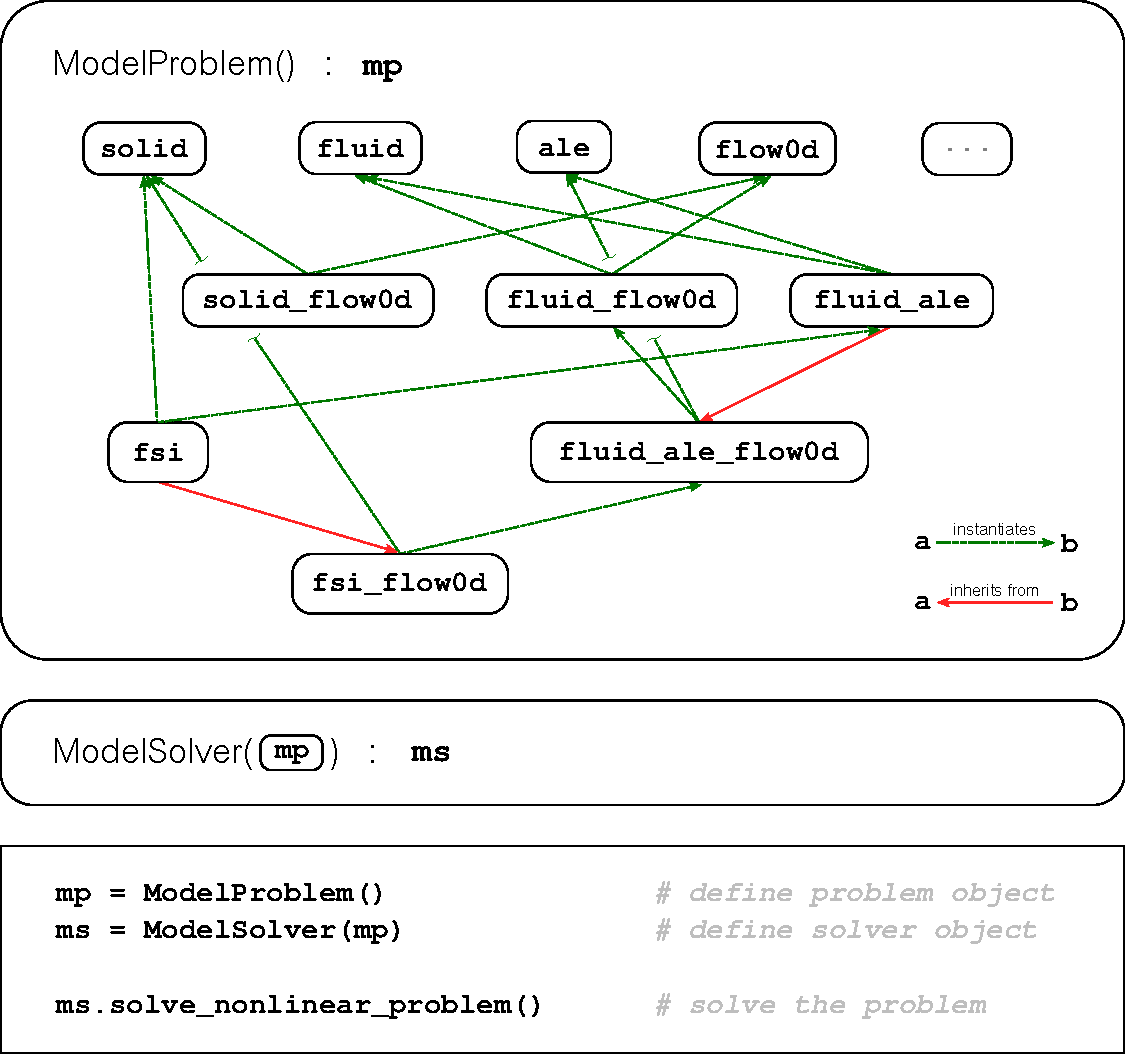
\includegraphics[width=0.8\textwidth]{/home/mh/work/publications/paper_ambit/code_design.pdf}
%\caption{Code design}\label{fig_code_design}
%\end{figure}

\section{Solid mechanics}\label{sec_solid}

-- Example: \verb.demos/solid.\\

-- Problem type: \verb.solid.\\

-- Solid mechanics are formulated in a Total Lagrangian frame

\subsection{Strong form}

\subsubsection{Displacement-based}
-- Primary variable: displacement $\bs{u}$
\begin{align}
\bs{\nabla}_{0} \cdot \bs{P}(\bs{u},\bs{v}(\bs{u})) + \hat{\bs{b}}_{0} &= \rho_{0} \bs{a}(\bs{u}) &&\text{in} \; \mathit{\Omega}_{0} \times [0, T], \label{eq_divP} \\
\bs{u} &= \hat{\bs{u}} &&\text{on} \; \mathit{\Gamma}_{0}^{\mathrm{D}} \times [0, T], \label{eq_bc_u}\\
\bs{t}_{0} = \bs{P}\bs{n}_{0} &= \hat{\bs{t}}_{0} &&\text{on} \; \mathit{\Gamma}_{0}^{\mathrm{N}} \times [0, T], \label{eq_bc_N}\\
\bs{u}(\bs{x}_{0},0) &= \hat{\bs{u}}_{0}(\bs{x}_{0}) &&\text{in} \; \mathit{\Omega}_{0}, \label{eq_ini_u}\\
\bs{v}(\bs{x}_{0},0) &= \hat{\bs{v}}_{0}(\bs{x}_{0}) &&\text{in} \; \mathit{\Omega}_{0}, \label{eq_ini_v}
\end{align}

\subsubsection{Incompressible mechanics}
-- Primary variables: displacement $\bs{u}$ and pressure $p$
\begin{align}
\bs{\nabla}_{0} \cdot \bs{P}(\bs{u},p,\bs{v}(\bs{u})) + \hat{\bs{b}}_{0} &= \rho_{0} \bs{a}(\bs{u}) &&\text{in} \; \mathit{\Omega}_{0} \times [0, T], \label{eq_divP_inc} \\
J(\bs{u})-1 &= 0 &&\text{in} \; \mathit{\Omega}_{0} \times [0, T], \label{eq_J} \\
\bs{u} &= \hat{\bs{u}} &&\text{on} \; \mathit{\Gamma}_{0}^{\mathrm{D}} \times [0, T], \label{eq_bc_u_inc}\\
\bs{t}_{0} = \bs{P}\bs{n}_{0} &= \hat{\bs{t}}_{0} &&\text{on} \; \mathit{\Gm}_{0}^{\mathrm{N}} \times [0, T], \label{eq_bc_N_inc}\\
\bs{u}(\bs{x}_{0},0) &= \hat{\bs{u}}_{0}(\bs{x}_{0}) &&\text{in} \; \mathit{\Om}_{0}, \label{eq_ini_u_inc}\\
\bs{v}(\bs{x}_{0},0) &= \hat{\bs{v}}_{0}(\bs{x}_{0}) &&\text{in} \; \mathit{\Om}_{0}, \label{eq_ini_v_inc}
\end{align}

with velocity and acceleration $\bs{v}=\frac{\mathrm{d}\bs{u}}{\mathrm{d}t}$ and $\bs{a}=\frac{\mathrm{d}^2\bs{u}}{\mathrm{d}t^2}$, respectively

\subsection{Weak form}

\subsubsection{Displacement-based}
-- Primary variable: displacement $\bs{u}$\\

-- Principal of Virtual Work:
\begin{align}
r(\bs{u};\delta\bs{u}) := \delta \mathcal{W}_{\mathrm{kin}}(\bs{u};\delta\bs{u}) + \delta \mathcal{W}_{\mathrm{int}}(\bs{u};\delta\bs{u}) - \delta \mathcal{W}_{\mathrm{ext}}(\bs{u};\delta\bs{u}) = 0, \quad \forall \; \delta\bs{u}\label{eq_res_u_solid}
\end{align}
-- Kinetic virtual work:
\begin{align}
\delta \mathcal{W}_{\mathrm{kin}}(\bs{u};\delta\bs{u}) &= \int\limits_{\Om_{0}} \rho_{0}\,\bs{a}(\bs{u}) \cdot \delta\bs{u} \,\mathrm{d}V \label{eq_deltaWkin}
\end{align}
-- Internal virtual work:
\begin{align}
\delta \mathcal{W}_{\mathrm{int}}(\bs{u};\delta\bs{u}) &= \int\limits_{\Om_{0}} \bs{P}(\bs{u},\bs{v}(\bs{u})) : \bs{\nabla}_{0} \delta\bs{u} \,\mathrm{d}V \label{eq_deltaWint}
\end{align}
-- External virtual work:\\
\begin{itemize}
\item conservative Neumann load:
\begin{align}
\delta \mathcal{W}_{\mathrm{ext}}(\delta\bs{u}) &= \int\limits_{\Gm_{0}^{\mathrm{N}}} \hat{\bs{t}}_{0}(t) \cdot \delta\bs{u} \,\mathrm{d}A \label{eq_deltaWext_pk1}
\end{align}
%add to the dict of boundary conditions:\\
%\adjustbox{width=.95\columnwidth}{%
%\verb\"neumann" : [{"id" : [<IDs>], "dir" : "xyz_ref", "curve" : [<#X>,<#Y>,<#Z>]}\
%}%
\item Neumann pressure load in current normal direction:
\begin{align}
\delta \mathcal{W}_{\mathrm{ext}}(\bs{u};\delta\bs{u}) &= -\int\limits_{\Gm_{0}^{\mathrm{N}}} \hat{p}(t)\,J \bs{F}^{-\mathrm{T}}\bs{n}_{0} \cdot \delta\bs{u} \,\mathrm{d}A \label{eq_deltaWext_cur_p}
\end{align}
\item general Neumann load in current direction:
\begin{align}
\delta \mathcal{W}_{\mathrm{ext}}(\bs{u};\delta\bs{u}) &= \int\limits_{\Gm_0} J\boldsymbol{F}^{-\mathrm{T}}\,\hat{\boldsymbol{t}}_{0}(t) \cdot \delta\boldsymbol{u} \,\mathrm{d}A \label{eq_deltaWext_cur}
\end{align}
\item body force:
\begin{align}
\delta \mathcal{W}_{\mathrm{ext}}(\delta\bs{u}) &= \int\limits_{\Om_{0}} \hat{\bs{b}}_{0}(t) \cdot \delta\bs{u} \,\mathrm{d}V \label{eq_deltaWext_body}
\end{align}

\item generalized Robin condition:
\begin{align}
\delta \mathcal{W}_{\mathrm{ext}}(\bs{u};\delta\bs{u}) &= -\int\limits_{\Gm_{0}^{\mathrm{N}}} \left[k\,\bs{u} + c\,\bs{v}(\bs{u})\right] \cdot \delta\bs{u}\,\mathrm{d}A \label{eq_deltaWext_rob}
\end{align} 
\item generalized Robin condition in reference surface normal direction:
\begin{align}
\delta \mathcal{W}_{\mathrm{ext}}(\bs{u};\delta\bs{u}) &= -\int\limits_{\Gm_{0}^{\mathrm{N}}} (\bs{n}_0 \otimes \bs{n}_0)\left[k\,\bs{u} + c\,\bs{v}(\bs{u})\right] \cdot \delta\bs{u}\,\mathrm{d}A \label{eq_deltaWext_robn}
\end{align}

\end{itemize}

-- Discrete nonlinear system to solve in each time step $n$:
\begin{align}
\left.\ROP_{u}(\bs{\mathsf{u}})\right|_{n+1} = \bs{\mathsf{0}}\label{eq_nonlin_sys_solid}
\end{align}

-- Discrete linear system to solve in each Newton iteration $k$:
\begin{align}
\left. \bs{\mathsf{K}}_{uu} \right|_{n+1}^{k} \Delta\bs{\mathsf{u}}_{n+1}^{k+1}=-\left. \ROP_{u} \right|_{n+1}^{k} \label{eq_lin_sys_solid}
\end{align}


\subsubsection{Incompressible mechanics: 2-field displacement and pressure variables}
-- Primary variables: displacement $\bs{u}$ and pressure $p$
\begin{align}
r_u(\bs{u},p;\delta\bs{u}) &:= \delta \mathcal{W}_{\mathrm{kin}}(\bs{u};\delta\bs{u}) + \delta \mathcal{W}_{\mathrm{int}}(\bs{u},p;\delta\bs{u}) - \delta \mathcal{W}_{\mathrm{ext}}(\bs{u};\delta\bs{u}) = 0, \quad \forall \; \delta\bs{u} \label{eq_res_u_solid_incomp}\\
r_p(\bs{u};\delta p) &:= \delta \mathcal{W}_{\mathrm{pres}}(\bs{u};\delta p) = 0, \quad \forall \; \delta p
\end{align}

-- Kinetic virtual work: (\ref{eq_deltaWkin})\\
-- Internal virtual work:
\begin{align}
\delta \mathcal{W}_{\mathrm{int}}(\bs{u},p;\delta\bs{u}) &= \int\limits_{\Om_{0}} \bs{P}(\bs{u},p,\bs{v}(\bs{u})) : \bs{\nabla}_{0} \delta\bs{u} \,\mathrm{d}V \label{eq_deltaWint_incomp}
\end{align}
-- Pressure virtual work:
\begin{align}
\delta \mathcal{W}_{\mathrm{pres}}(\bs{u};\delta p) &= \int\limits_{\Om_{0}} (J(\bs{u}) - 1) \,\delta p \,\mathrm{d}V \label{eq_deltaWpres}
\end{align}

-- Discrete nonlinear system to solve in each time step $n$:
\begin{align}
\ROP_{n+1} = \begin{bmatrix} \ROP_{u}(\bs{\mathsf{u}},\bs{\mathsf{p}}) \\ \ROP_{p}(\bs{\mathsf{u}}) \end{bmatrix}_{n+1} = \bs{\mathsf{0}}\label{eq_nonlin_sys_solid_inc}
\end{align}

-- Discrete linear system to solve in each Newton iteration $k$:
\begin{align}
\begin{bmatrix} \bs{\mathsf{K}}_{uu} & \bs{\mathsf{K}}_{up} \\ \\ \bs{\mathsf{K}}_{pu} & \zerom \end{bmatrix}_{n+1}^{k}\begin{bmatrix} \Delta\bs{\mathsf{u}} \\ \\ \Delta\bs{\mathsf{p}} \end{bmatrix}_{n+1}^{k+1}=-\begin{bmatrix} \ROP_{u} \\ \\ \ROP_{p} \end{bmatrix}_{n+1}^{k} \label{eq_lin_sys_solid_incomp}
\end{align}


\section{Fluid mechanics}\label{sec_fluid}

\subsection{Eulerian reference frame}\label{subsec_fluid_eulerian}

-- Example: \verb.demos/fluid.\\

-- Problem type: \verb.fluid.\\

-- Incompressible Navier-Stokes equations in Eulerian reference frame\\

\subsubsection{Strong Form}
-- Primary variables: velocity $\bs{v}$ and pressure $p$
\begin{align}
\bs{\nabla} \cdot \bs{\sigma}(\bs{v},p) + \hat{\bs{b}} &= \rho\left(\frac{\partial\bs{v}}{\partial t} + (\bs{\nabla}\bs{v})\,\bs{v}\right) &&\text{in} \; \mathit{\Om}_t \times [0, T], \label{eq_divsigma_ns} \\
\bs{\nabla}\cdot \bs{v} &= 0 &&\text{in} \; \mathit{\Om}_t \times [0, T],\label{eq_divv_ns}\\
\bs{v} &= \hat{\bs{v}} &&\text{on} \; \mathit{\Gm}_t^{\mathrm{D}} \times [0, T], \label{eq_bc_v_ns}\\
\bs{t} = \bs{\sigma}\bs{n} &= \hat{\bs{t}} &&\text{on} \; \mathit{\Gm}_t^{\mathrm{N}} \times [0, T], \label{eq_bc_N_ns}\\
\bs{v}(\bs{x},0) &= \hat{\bs{v}}_{0}(\bs{x}) &&\text{in} \; \mathit{\Om}_t, \label{eq_ini_v_ns}
\end{align}

with a Newtonian fluid constitutive law
\begin{align}
\bs{\sigma} = -p \bs{I} + 2 \mu\,\bs{\gamma} = -p \bs{I} + \mu \left(\bs{\nabla} \bs{v} + (\bs{\nabla} \bs{v})^{\mathrm{T}}\right)
\end{align}

\subsubsection{Weak Form}
-- Primary variables: velocity $\bs{v}$ and pressure $p$\\

-- Principle of Virtual Power
\begin{align}
r_v(\bs{v},p;\delta\bs{v}) &:= \delta \mathcal{P}_{\mathrm{kin}}(\bs{v};\delta\bs{v}) + \delta \mathcal{P}_{\mathrm{int}}(\bs{v},p;\delta\bs{v}) - \delta \mathcal{P}_{\mathrm{ext}}(\bs{v};\delta\bs{v}) = 0, \quad \forall \; \delta\bs{v} \label{eq_res_v_fluid}\\
r_p(\bs{v};\delta p) &:= \delta \mathcal{P}_{\mathrm{pres}}(\bs{v};\delta p), \quad \forall \; \delta p \label{eq_res_p_fluid}
\end{align}

-- Kinetic virtual power:
\begin{align}
\delta \mathcal{P}_{\mathrm{kin}}(\bs{v};\delta\bs{v}) = \int\limits_{\Om_t} \rho\left(\frac{\partial\bs{v}}{\partial t} + (\bs{\nabla}\bs{v})\,\bs{v}\right) \cdot \delta\bs{v} \,\mathrm{d}v
\end{align}
-- Internal virtual power:
\begin{align}
\delta \mathcal{P}_{\mathrm{int}}(\bs{v},p;\delta\bs{v}) = 
\int\limits_{\Om_t} \bs{\sigma}(\bs{v},p) : \bs{\nabla} \delta\bs{v} \,\mathrm{d}v 
\end{align}

-- Pressure virtual power:
\begin{align}
\delta \mathcal{P}_{\mathrm{pres}}(\bs{v};\delta p) = 
\int\limits_{\Om_t} (\bs{\nabla}\cdot\bs{v})\,\delta p\,\mathrm{d}v
\end{align}

-- External virtual power:\\
\begin{itemize}
\item conservative Neumann load:
\begin{align}
\delta \mathcal{P}_{\mathrm{ext}}(\delta\bs{v}) &= \int\limits_{\Gm_t^{\mathrm{N}}} \hat{\bs{t}}(t) \cdot \delta\bs{v} \,\mathrm{d}a \label{eq_deltaPext_neumann}
\end{align}
\item pressure Neumann load:
\begin{align}
\delta \mathcal{P}_{\mathrm{ext}}(\delta\bs{v}) &= -\int\limits_{\Gm_t^{\mathrm{N}}} \hat{p}(t)\,\bs{n} \cdot \delta\bs{v} \,\mathrm{d}a \label{eq_deltaPext_neumann_true}
\end{align}
\item body force:
\begin{align}
\delta \mathcal{P}_{\mathrm{ext}}(\delta\bs{v}) &= \int\limits_{\Om_t} \hat{\bs{b}}(t) \cdot \delta\bs{v} \,\mathrm{d}V \label{eq_deltaPext_body}
\end{align}
\end{itemize}

\subsubsection{Stabilization}\label{subsubsec_stab}
Streamline-upwind Petrov-Galerkin/pressure-stabilizing Petrov-Galerkin (SUPG/PSPG) methods are implemented, either using the full or a reduced scheme\\

Full scheme according to \cite{tezduyar2000}: \verb.supg_pspg.:\\
-- Velocity residual operator (\ref{eq_res_v_fluid}) is augmented with the following terms:
\begin{align}
r_v \leftarrow r_v &+ \frac{1}{\rho}\int\limits_{\Om_t} \tau_{\mathrm{SUPG}}\,(\bs{\nabla}\delta\bs{v})\,\bs{v} \cdot \left[\rho\left(\frac{\partial \bs{v}}{\partial t} + (\bs{\nabla}\bs{v})\,\bs{v}\right) - \bs{\nabla} \cdot \bs{\sigma}(\bs{v},p)\right]\,\mathrm{d}v \\
& + \int\limits_{\Om_t} \tau_{\mathrm{LSIC}}\,\rho\,(\bs{\nabla}\cdot\delta\bs{v})(\bs{\nabla}\cdot\bs{v})\,\mathrm{d}v
\end{align}
-- Pressure residual operator (\ref{eq_res_p_fluid}) is augmented with the following terms:
\begin{align}
r_p \leftarrow r_p &+ \frac{1}{\rho}\int\limits_{\Om_t} \tau_{\mathrm{PSPG}}\,(\bs{\nabla}\delta p) \cdot \left[\rho\left(\frac{\partial \bs{v}}{\partial t} + (\bs{\nabla}\bs{v})\,\bs{v}\right) - \bs{\nabla} \cdot \bs{\sigma}(\bs{v},p)\right]\,\mathrm{d}v 
\end{align}


Reduced scheme (optimized for first-order): \verb.supg_pspg2.:

-- Velocity residual operator (\ref{eq_res_v_fluid}) is augmented with the following terms:
\begin{align}
r_v \leftarrow r_v &+ \int\limits_{\Om_t} d_1\,((\bs{\nabla}\bs{v})\,\bs{v}) \cdot (\bs{\nabla}\delta\bs{v})\,\bs{v}\,\mathrm{d}v \\
& + \int\limits_{\Om_t} d_2\,(\bs{\nabla}\cdot\bs{v}) (\bs{\nabla}\cdot\delta\bs{v})\,\mathrm{d}v\\
&+ \int\limits_{\Om_t} d_3\,(\bs{\nabla}p) \cdot (\bs{\nabla}\delta\bs{v})\,\bs{v}\,\mathrm{d}v 
\end{align}
-- Pressure residual operator (\ref{eq_res_p_fluid}) is augmented with the following terms:
\begin{align}
r_p \leftarrow r_p &+ \frac{1}{\rho}\int\limits_{\Om_t} d_1\,((\bs{\nabla}\bs{v})\,\bs{v}) \cdot (\bs{\nabla}\delta p)\,\mathrm{d}v \\
&+ \frac{1}{\rho}\int\limits_{\Om_t} d_3\,(\bs{\nabla}p) \cdot (\bs{\nabla}\delta p)\,\mathrm{d}v 
\end{align}

-- Discrete nonlinear system to solve in each time step $n$:
\begin{align}
\ROP_{n+1} = \begin{bmatrix} \ROP_{v}(\bs{\mathsf{v}},\bs{\mathsf{p}}) \\ \ROP_{p}(\bs{\mathsf{p}},\bs{\mathsf{v}}) \end{bmatrix}_{n+1} = \bs{\mathsf{0}}\label{eq_nonlin_sys_fluid}
\end{align}

-- Discrete linear system to solve in each Newton iteration $k$:
\begin{align}
\begin{bmatrix} \bs{\mathsf{K}}_{vv} & \bs{\mathsf{K}}_{vp} \\ \\ \bs{\mathsf{K}}_{pv} & \bs{\mathsf{K}}_{pp} \end{bmatrix}_{n+1}^{k}\begin{bmatrix} \Delta\bs{\mathsf{v}} \\ \\ \Delta\bs{\mathsf{p}} \end{bmatrix}_{n+1}^{k+1}=-\begin{bmatrix} \ROP_{v} \\ \\ \ROP_{p} \end{bmatrix}_{n+1}^{k} \label{eq_lin_sys_fluid}
\end{align}
-- Note that $\bs{\mathsf{K}}_{pp}$ is zero for Taylor-Hood elements (without stabilization)

\subsection{ALE reference frame}

-- Problem type: \verb.fluid_ale.\\

-- Incompressible Navier-Stokes equations in Arbitrary Lagrangian Eulerian (ALE) reference frame\\

-- ALE domain problem deformation governed by linear-elastic or nonlinear hyperelastic solid, displacement field $\bs{d}$\\

-- Fluid mechanics formulated with respect to the reference frame, using ALE deformation gradient $\bs{F}(\bs{d}) = \bs{I} + \bs{\nabla}_0\bs{d}$ and its determinant, $J(\bs{d})=\det \bs{F}(\bs{d})$\\

\subsubsection{ALE problem}

-- Displacement-based quasi-static solid\\

-- Primary variable: domain displacement $\bs{d}$\\

-- Strong form:
\begin{align}
\bs{\nabla}_{0} \cdot \bs{\sigma}^{\mathrm{G}}(\bs{d}) &= \bs{0} &&\text{in} \; \mathit{\Om}_0, \label{eq_divsigma_ale} \\
\bs{d} &= \hat{\bs{d}} &&\text{on} \; \mathit{\Gm}_0^{\mathrm{D}}, \label{eq_dbc_ale}
\end{align}
with
\begin{align}
\bs{\sigma}^{\mathrm{G}}(\bs{d}) = E \,\frac{1}{2}\left(\bs{\nabla}_0\bs{d} + (\bs{\nabla}_0\bs{d})^{\mathrm{T}}\right) + \kappa \left(\bs{\nabla}_0 \cdot \bs{d}\right)\,\bs{I}
\end{align}

-- weak form:
\begin{align}
r_{d}(\bs{d};\delta\bs{d}) := \int\limits_{\Om_0}\bs{\sigma}^{\mathrm{G}}(\bs{d}) : \bs{\nabla}_{0}\delta\bs{d}\,\mathrm{d}V = 0, \quad \forall \; \delta\bs{d} \label{eq_r_d}
\end{align}


\subsubsection{Strong form}
-- Primary variables: velocity $\bs{v}$, pressure $p$, and domain displacement $\bs{d}$
\begin{align}
\bs{\nabla}_{0} \bs{\sigma}(\bs{v},\bs{d},p) : \bs{F}^{-\mathrm{T}} + \hat{\bs{b}} &= \rho\left(\frac{\partial\bs{v}}{\partial t} + (\bs{\nabla}_0\bs{v}\,\bs{F}^{-1})\,\bs{v}\right) &&\text{in} \; \mathit{\Om}_0 \times [0, T], \label{eq_divsigma_ns_ale} \\
\bs{\nabla}_{0}\bs{v} : \bs{F}^{-\mathrm{T}} &= 0 &&\text{in} \; \mathit{\Om}_0 \times [0, T],\label{eq_divv_ns_ale}\\
\bs{v} &= \hat{\bs{v}} &&\text{on} \; \mathit{\Gm}_0^{\mathrm{D}} \times [0, T], \label{eq_bc_v_ns_ale}\\
\bs{t} = \bs{\sigma}\bs{n} &= \hat{\bs{t}} &&\text{on} \; \mathit{\Gm}_0^{\mathrm{N}} \times [0, T], \label{eq_bc_N_ns_ale}\\
\bs{v}(\bs{x},0) &= \hat{\bs{v}}_{0}(\bs{x}) &&\text{in} \; \mathit{\Om}_0, \label{eq_ini_v_ns_ale}
\end{align}

with a Newtonian fluid constitutive law
\begin{align}
\bs{\sigma} = -p \bs{I} + 2 \mu \bs{\gamma} = -p \bs{I} + \mu \left(\bs{\nabla}_0 \bs{v}\,\bs{F}^{-1} + \bs{F}^{-\mathrm{T}}(\bs{\nabla}_0 \bs{v})^{\mathrm{T}}\right)
\end{align}

\subsubsection{Weak form}

-- Primary variables: velocity $\bs{v}$, pressure $p$, and domain displacement $\bs{d}$\\

-- Principle of Virtual Power
\begin{align}
r_v(\bs{v},p,\bs{d};\delta\bs{v}) &:= \delta \mathcal{P}_{\mathrm{kin}}(\bs{v},\bs{d};\delta\bs{v}) + \delta \mathcal{P}_{\mathrm{int}}(\bs{v},p,\bs{d};\delta\bs{v}) - \delta \mathcal{P}_{\mathrm{ext}}(\bs{v},\bs{d};\delta\bs{v}) = 0, \quad \forall \; \delta\bs{v} \label{eq_res_v_fluid_ale}\\
r_p(\bs{v},\bs{d};\delta p) &:= \delta \mathcal{P}_{\mathrm{pres}}(\bs{v},\bs{d};\delta p), \quad \forall \; \delta p \label{eq_res_p_fluid_ale}
\end{align}

-- Kinetic virtual power:
\begin{align}
\delta \mathcal{P}_{\mathrm{kin}}(\bs{v},\bs{d};\delta\bs{v}) = \int\limits_{\Om_0} J \rho\left(\frac{\partial\bs{v}}{\partial t} + (\bs{\nabla}_{0}\bs{v}\,\bs{F}^{-1})\,\bs{v}\right) \cdot \delta\bs{v} \,\mathrm{d}V
\end{align}
-- Internal virtual power:
\begin{align}
\delta \mathcal{P}_{\mathrm{int}}(\bs{v},p,\bs{d};\delta\bs{v}) = 
\int\limits_{\Om_0} J\bs{\sigma}(\bs{v},p,\bs{d}) : \bs{\nabla}_{0} \delta\bs{v}\,\bs{F}^{-1} \,\mathrm{d}V
\end{align}

-- Pressure virtual power:
\begin{align}
\delta \mathcal{P}_{\mathrm{pres}}(\bs{v},\bs{d};\delta p) = 
\int\limits_{\Om_0} J\,\bs{\nabla}_{0}\bs{v} : \bs{F}^{-\mathrm{T}}\delta p\,\mathrm{d}V
\end{align}

-- External virtual power:\\
\begin{itemize}
\item conservative Neumann load:
\begin{align}
\delta \mathcal{P}_{\mathrm{ext}}(\delta\bs{v}) &= \int\limits_{\Gm_0^{\mathrm{N}}} \hat{\bs{t}}(t) \cdot \delta\bs{v} \,\mathrm{d}A \label{eq_deltaPext_neumann_ale}
\end{align}
\item pressure Neumann load:
\begin{align}
\delta \mathcal{P}_{\mathrm{ext}}(\bs{d};\delta\bs{v}) &= -\int\limits_{\Gm_0^{\mathrm{N}}} \hat{p}(t)\,J\bs{F}^{-\mathrm{T}}\bs{n}_{0} \cdot \delta\bs{v} \,\mathrm{d}A \label{eq_deltaPext_neumann_ale_true}
\end{align}
\item body force:
\begin{align}
\delta \mathcal{P}_{\mathrm{ext}}(\bs{d};\delta\bs{v}) &= \int\limits_{\Om_0} J\,\hat{\bs{b}}(t) \cdot \delta\bs{v} \,\mathrm{d}V \label{eq_deltaPext_body_ale}
\end{align}
\end{itemize}

\subsubsection{Stabilization}
ALE forms of stabilization introduced in sec. \ref{subsubsec_stab}\\
\verb.supg_pspg.:\\
-- Velocity residual operator (\ref{eq_res_v_fluid_ale}) is augmented with the following terms:
\begin{align}
r_v \leftarrow r_v &+ \frac{1}{\rho}\int\limits_{\Om_0}J\, \tau_{\mathrm{SUPG}}\,(\bs{\nabla}_0\delta\bs{v}\,\bs{F}^{-1})\,\bs{v}\;\cdot \\
& \qquad\quad \cdot\left[\rho\left(\frac{\partial \bs{v}}{\partial t} + (\bs{\nabla}_0\bs{v}\,\bs{F}^{-1})\,(\bs{v}-\bs{w})\right) - \bs{\nabla}_{0} \bs{\sigma}(\bs{v},\bs{d},p) : \bs{F}^{-\mathrm{T}}\right]\,\mathrm{d}V \\
& + \int\limits_{\Om_0}J\, \tau_{\mathrm{LSIC}}\,\rho\,(\bs{\nabla}_{0}\delta\bs{v} : \bs{F}^{-\mathrm{T}})(\bs{\nabla}_{0}\bs{v} : \bs{F}^{-\mathrm{T}})\,\mathrm{d}V
\end{align}
-- Pressure residual operator (\ref{eq_res_p_fluid_ale}) is augmented with the following terms:
\begin{align}
r_p \leftarrow r_p &+ \frac{1}{\rho}\int\limits_{\Om_0}J\, \tau_{\mathrm{PSPG}}\,(\bs{F}^{-\mathrm{T}}\bs{\nabla}_{0}\delta p) \;\cdot \\
& \qquad\quad \cdot \left[\rho\left(\frac{\partial \bs{v}}{\partial t} + (\bs{\nabla}_0\bs{v}\,\bs{F}^{-1})\,(\bs{v}-\bs{w})\right) - \bs{\nabla}_{0} \bs{\sigma}(\bs{v},\bs{d},p) : \bs{F}^{-\mathrm{T}}\right]\,\mathrm{d}V
\end{align}

\verb.supg_pspg2.:\\
-- Velocity residual operator (\ref{eq_res_v_fluid_ale}) is augmented with the following terms:
\begin{align}
r_v \leftarrow r_v &+ \int\limits_{\Om_0} J\,d_1\,((\bs{\nabla}_{0}\bs{v}\,\bs{F}^{-1})\,(\bs{v}-\bs{w})) \cdot (\bs{\nabla}_{0}\delta\bs{v}\,\bs{F}^{-1})\,\bs{v}\,\mathrm{d}V \\
& + \int\limits_{\Om_0} J\,d_2\,(\bs{\nabla}_{0}\bs{v} : \bs{F}^{-\mathrm{T}}) (\bs{\nabla}_{0}\delta\bs{v} : \bs{F}^{-\mathrm{T}})\,\mathrm{d}V\\
&+ \int\limits_{\Om_0} J\,d_3\,(\bs{F}^{-\mathrm{T}}\bs{\nabla}_{0}p) \cdot (\bs{\nabla}_{0}\delta\bs{v}\,\bs{F}^{-1})\,\bs{v}\,\mathrm{d}V
\end{align}
-- Pressure residual operator (\ref{eq_res_p_fluid_ale}) is augmented with the following terms:
\begin{align}
r_p \leftarrow r_p &+ \frac{1}{\rho}\int\limits_{\Om_0} J\,d_1\,((\bs{\nabla}_{0}\bs{v}\,\bs{F}^{-1})\,(\bs{v}-\bs{w})) \cdot (\bs{F}^{-\mathrm{T}}\bs{\nabla}_{0}\delta p)\,\mathrm{d}V \\
&+ \frac{1}{\rho}\int\limits_{\Om_0} J\,d_3\,(\bs{F}^{-\mathrm{T}}\bs{\nabla}_{0}p) \cdot (\bs{F}^{-\mathrm{T}}\bs{\nabla}_{0}\delta p)\,\mathrm{d}V
\end{align}

-- Discrete nonlinear system to solve in each time step $n$:
\begin{align}
\ROP_{n+1} = \begin{bmatrix} \ROP_{v}(\bs{\mathsf{v}},\bs{\mathsf{p}},\bs{\mathsf{d}}) \\ \ROP_{p}(\bs{\mathsf{p}},\bs{\mathsf{v}},\bs{\mathsf{d}}) \\ \ROP_{d}(\bs{\mathsf{d}}) \end{bmatrix}_{n+1} = \bs{\mathsf{0}}\label{eq_nonlin_sys_fluid_ale}
\end{align}

-- Discrete linear system to solve in each Newton iteration $k$:
\begin{align}
\begin{bmatrix} \bs{\mathsf{K}}_{vv} & \bs{\mathsf{K}}_{vp} & \bs{\mathsf{K}}_{vd} \\ \\ \bs{\mathsf{K}}_{pv} & \bs{\mathsf{K}}_{pp} & \bs{\mathsf{K}}_{pd} \\ \\ \bs{\mathsf{K}}_{dv}  & \zerom & \bs{\mathsf{K}}_{dd} \end{bmatrix}_{n+1}^{k}\begin{bmatrix} \Delta\bs{\mathsf{v}} \\ \\ \Delta\bs{\mathsf{p}} \\ \\ \Delta\bs{\mathsf{d}} \end{bmatrix}_{n+1}^{k+1}=-\begin{bmatrix} \ROP_{v} \\ \\ \ROP_{p} \\ \\ \ROP_{d} \end{bmatrix}_{n+1}^{k} \label{eq_lin_sys_fluid_ale}
\end{align}
-- note that $\bs{\mathsf{K}}_{pp}$ is zero for Taylor-Hood elements (without stabilization)


\section{0D flow: Lumped parameter models}\label{sec_flow0d}

-- Example: \verb.demos/flow0d.\\

-- Problem type: \verb.flow0d.\\

\subsection{2-element Windkessel}

- Model type : \verb.2elwindkessel.\\

\subsection{4-element Windkessel (inertance parallel to impedance)}

- Model type : \verb.4elwindkesselLpZ.\\

\subsection{4-element Windkessel (inertance serial to impedance)}

- Model type : \verb.4elwindkesselLsZ.\\

\subsection{Systemic and pulmonary circulation}

- Model type : \verb.syspul.\\

- Allows to link in a coronary flow model

\begin{align}
&\text{left heart and systemic circulation} && \nonumber\\
&-Q_{\mathrm{at}}^{\ell} = \sum\limits_{i=1}^{n_{\mathrm{ven}}^{\mathrm{pul}}}q_{\mathrm{ven},i}^{\mathrm{pul}} - q_{\mathrm{v,in}}^{\ell} && \text{left atrium flow balance}\nonumber\\
&q_{\mathrm{v,in}}^{\ell} = q_{\mathrm{mv}}(p_{\mathrm{at}}^{\ell}-p_{\mathrm{v}}^{\ell}) && \text{mitral valve momentum}\label{eq_mv_flow}\\
&-Q_{\mathrm{v}}^{\ell} = q_{\mathrm{v,in}}^{\ell} - q_{\mathrm{v,out}}^{\ell} && \text{left ventricle flow balance}\nonumber\\
&q_{\mathrm{v,out}}^{\ell} = q_{\mathrm{av}}(p_{\mathrm{v}}^{\ell}-p_{\mathrm{ar}}^{\mathrm{sys}}) && \text{aortic valve momentum}\label{eq_av_flow}\\
&-Q_{\mathrm{aort}}^{\mathrm{sys}} = q_{\mathrm{v,out}}^{\ell} - q_{\mathrm{ar,p}}^{\mathrm{sys}} - \mathbb{I}^{\mathrm{cor}}\sum\limits_{i=1}^{2}q_{\mathrm{ar,cor,in},i}^{\mathrm{sys}} && \text{aortic root flow balance}\nonumber\\
&I_{\mathrm{ar}}^{\mathrm{sys}} \frac{\mathrm{d}q_{\mathrm{ar,p}}^{\mathrm{sys}}}{\mathrm{d}t} + Z_{\mathrm{ar}}^{\mathrm{sys}}\,q_{\mathrm{ar,p}}^{\mathrm{sys}}=p_{\mathrm{ar}}^{\mathrm{sys}}-p_{\mathrm{ar,d}}^{\mathrm{sys}} && \text{aortic root inertia}\nonumber\\
&C_{\mathrm{ar}}^{\mathrm{sys}} \frac{\mathrm{d}p_{\mathrm{ar,d}}^{\mathrm{sys}}}{\mathrm{d}t} = q_{\mathrm{ar,p}}^{\mathrm{sys}} - q_{\mathrm{ar}}^{\mathrm{sys}} && \text{systemic arterial flow balance}\nonumber\\
&L_{\mathrm{ar}}^{\mathrm{sys}} \frac{\mathrm{d}q_{\mathrm{ar}}^{\mathrm{sys}}}{\mathrm{d}t} + R_{\mathrm{ar}}^{\mathrm{sys}}\,q_{\mathrm{ar}}^{\mathrm{sys}}=p_{\mathrm{ar,d}}^{\mathrm{sys}}-p_{\mathrm{ven}}^{\mathrm{sys}} && \text{systemic arterial momentum}\nonumber\\
&C_{\mathrm{ven}}^{\mathrm{sys}} \frac{\mathrm{d}p_{\mathrm{ven}}^{\mathrm{sys}}}{\mathrm{d}t} = q_{\mathrm{ar}}^{\mathrm{sys}}-\sum\limits_{i=1}^{n_{\mathrm{ven}}^{\mathrm{sys}}}q_{\mathrm{ven},i}^{\mathrm{sys}}\ && \text{systemic venous flow balance}\nonumber\\
&L_{\mathrm{ven},i}^{\mathrm{sys}} \frac{\mathrm{d}q_{\mathrm{ven},i}^{\mathrm{sys}}}{\mathrm{d}t} + R_{\mathrm{ven},i}^{\mathrm{sys}}\, q_{\mathrm{ven},i}^{\mathrm{sys}} = p_{\mathrm{ven}}^{\mathrm{sys}} - p_{\mathrm{at},i}^{r} && \text{systemic venous momentum}\nonumber\\
&\qquad\qquad i \in \{1,...,n_{\mathrm{ven}}^{\mathrm{sys}}\} && \nonumber
\end{align}
\begin{align}
&\text{right heart and pulmonary circulation} && \nonumber\\
&-Q_{\mathrm{at}}^{r} = \sum\limits_{i=1}^{n_{\mathrm{ven}}^{\mathrm{sys}}}q_{\mathrm{ven},i}^{\mathrm{sys}} - \mathbb{I}^{\mathrm{cor}} q_{\mathrm{ven,cor,out}}^{\mathrm{sys}} - q_{\mathrm{v,in}}^{r} && \text{right atrium flow balance}\nonumber\\
&q_{\mathrm{v,in}}^{r} = q_{\mathrm{tv}}(p_{\mathrm{at}}^{r}-p_{\mathrm{v}}^{r}) && \text{tricuspid valve momentum}\label{eq_tv_flow}\\
&-Q_{\mathrm{v}}^{r} = q_{\mathrm{v,in}}^{r} - q_{\mathrm{v,out}}^{r} && \text{right ventricle flow balance}\nonumber\\
&q_{\mathrm{v,out}}^{r} = q_{\mathrm{pv}}(p_{\mathrm{v}}^{r}-p_{\mathrm{ar}}^{\mathrm{pul}}) && \text{pulmonary valve momentum}\label{eq_pv_flow}\\
&C_{\mathrm{ar}}^{\mathrm{pul}} \frac{\mathrm{d}p_{\mathrm{ar}}^{\mathrm{pul}}}{\mathrm{d}t} = q_{\mathrm{v,out}}^{r} - q_{\mathrm{ar}}^{\mathrm{pul}} && \text{pulmonary arterial flow balance}\nonumber\\
&L_{\mathrm{ar}}^{\mathrm{pul}} \frac{\mathrm{d}q_{\mathrm{ar}}^{\mathrm{pul}}}{\mathrm{d}t} + R_{\mathrm{ar}}^{\mathrm{pul}}\,q_{\mathrm{ar}}^{\mathrm{pul}}=p_{\mathrm{ar}}^{\mathrm{pul}} -p_{\mathrm{ven}}^{\mathrm{pul}} && \text{pulmonary arterial momentum}\nonumber\\
&C_{\mathrm{ven}}^{\mathrm{pul}} \frac{\mathrm{d}p_{\mathrm{ven}}^{\mathrm{pul}}}{\mathrm{d}t} = q_{\mathrm{ar}}^{\mathrm{pul}} - \sum\limits_{i=1}^{n_{\mathrm{ven}}^{\mathrm{pul}}}q_{\mathrm{ven},i}^{\mathrm{pul}} && \text{pulmonary venous flow balance}\nonumber\\
&L_{\mathrm{ven},i}^{\mathrm{pul}} \frac{\mathrm{d}q_{\mathrm{ven},i}^{\mathrm{pul}}}{\mathrm{d}t} + R_{\mathrm{ven},i}^{\mathrm{pul}}\, q_{\mathrm{ven},i}^{\mathrm{pul}}=p_{\mathrm{ven}}^{\mathrm{pul}}-p_{\mathrm{at},i}^{\ell} && \text{pulmonary venous momentum}\nonumber\\
&\qquad\qquad i \in \{1,...,n_{\mathrm{ven}}^{\mathrm{pul}}\} && \nonumber
\end{align}

with:
\begin{align}
Q_{\mathrm{at}}^{\ell} := -\frac{\mathrm{d}V_{\mathrm{at}}^{\ell}}{\mathrm{d}t}, \quad
Q_{\mathrm{v}}^{\ell} := -\frac{\mathrm{d}V_{\mathrm{v}}^{\ell}}{\mathrm{d}t}, \quad
Q_{\mathrm{at}}^{r} := -\frac{\mathrm{d}V_{\mathrm{at}}^{r}}{\mathrm{d}t}, \quad
Q_{\mathrm{v}}^{r} := -\frac{\mathrm{d}V_{\mathrm{v}}^{r}}{\mathrm{d}t},
\quad
Q_{\mathrm{aort}}^{\mathrm{sys}} := -\frac{\mathrm{d}V_{\mathrm{aort}}^{\mathrm{sys}}}{\mathrm{d}t}\nonumber
\end{align}

and:
\begin{align}
\mathbb{I}^{\mathrm{cor}} = \begin{cases} 1, & \text{if \, CORONARY\_MODEL}, \\ 0, & \text{else} \end{cases}\nonumber
\end{align}

The volume $V$ of the heart chambers (0D) is modeled by the volume-pressure relationship
\begin{equation}
V(t) = \frac{p}{E(t)} + V_{\mathrm{u}},
\end{equation}
with the unstressed volume $V_{\mathrm{u}}$ and the time-varying elastance
\begin{equation}
E(t)=\left(E_{\mathrm{max}}-E_{\mathrm{min}}\right)\cdot \hat{y}(t)+E_{\mathrm{min}} \label{at_elast},
\end{equation}
where $E_{\mathrm{max}}$ and $E_{\mathrm{min}}$ denote the maximum and minimum elastance, respectively. The normalized activation function $\hat{y}(t)$ is input by the user.

Flow-pressure relations for the four valves, eq. (\ref{eq_mv_flow}), (\ref{eq_av_flow}), (\ref{eq_tv_flow}), (\ref{eq_pv_flow}), are functions of the pressure difference $p-p_{\mathrm{open}}$ across the valve. The following valve models can be defined:

Valve model \verb.pwlin_pres.:
\begin{align}
q(p-p_{\mathrm{open}}) = \frac{p-p_{\mathrm{open}}}{\tilde{R}}, \quad \text{with}\; \tilde{R} = \begin{cases} R_{\max}, & p < p_{\mathrm{open}} \\
R_{\min}, & p \geq p_{\mathrm{open}} \end{cases}\nonumber
\end{align}
\textbf{Remark:} Non-smooth flow-pressure relationship

Valve model \verb.pwlin_time.:
\begin{align}
q(p-p_{\mathrm{open}}) = \frac{p-p_{\mathrm{open}}}{\tilde{R}},\quad \text{with}\; \tilde{R} = \begin{cases} \begin{cases} R_{\max}, & t < t_{\mathrm{open}} \;\text{and}\; t \geq t_{\mathrm{close}} \\
R_{\min}, & t \geq t_{\mathrm{open}} \;\text{or}\; t < t_{\mathrm{close}} \end{cases}, & t_{\mathrm{open}} > t_{\mathrm{close}} \\ \begin{cases} R_{\max}, & t < t_{\mathrm{open}} \;\text{or}\; t \geq t_{\mathrm{close}} \\
R_{\min}, & t \geq t_{\mathrm{open}} \;\text{and}\; t < t_{\mathrm{close}} \end{cases}, & \text{else} \end{cases}\nonumber
\end{align}
\textbf{Remark:} Non-smooth flow-pressure relationship with resistance only dependent on timings, not the pressure difference!

Valve model \verb.smooth_pres_resistance.:
\begin{align}
q(p-p_{\mathrm{open}}) = \frac{p-p_{\mathrm{open}}}{\tilde{R}},\quad \text{with}\;\tilde{R} = 0.5\left(R_{\max}-R_{\min}\right)\left(\tanh\frac{p-p_{\mathrm{open}}}{\epsilon}+1\right) + R_{\min}\nonumber
\end{align}
\textbf{Remark:} Smooth but potentially non-convex flow-pressure relationship!

Valve model \verb.smooth_pres_momentum.:
\begin{align}
q(p-p_{\mathrm{open}}) = \begin{cases}\frac{p-p_{\mathrm{open}}}{R_{\max}}, & p < p_{\mathrm{open}}-0.5\epsilon \\ h_{00}p_{0} + h_{10}m_{0}\epsilon + h_{01}p_{1} + h_{11}m_{1}\epsilon, & p \geq p_{\mathrm{open}}-0.5\epsilon \;\text{and}\; p < p_{\mathrm{open}}+0.5\epsilon \\ \frac{p-p_{\mathrm{open}}}{R_{\min}}, & p \geq p_{\mathrm{open}}+0.5\epsilon  \end{cases}\nonumber
\end{align}
with
\begin{align}
p_{0}=\frac{-0.5\epsilon}{R_{\max}}, \qquad m_{0}=\frac{1}{R_{\max}}, \qquad && p_{1}=\frac{0.5\epsilon}{R_{\min}}, \qquad m_{1}=\frac{1}{R_{\min}} \nonumber
\end{align}
and
\begin{align}
h_{00}=2s^3 - 3s^2 + 1, &\qquad h_{01}=-2s^3 + 3s^2, \nonumber\\
h_{10}=s^3 - 2s^2 + s, &\qquad h_{11}=s^3 - s^2 \nonumber
\end{align}
with
\begin{align}
s=\frac{p-p_{\mathrm{open}}+0.5\epsilon}{\epsilon} \nonumber
\end{align}
\textbf{Remarks:}\\
$-$ Collapses to valve model \verb.pwlin_pres. for $\epsilon=0$\\
$-$ Smooth and convex flow-pressure relationship

Valve model \verb.pw_pres_regurg.:
\begin{equation}
q(p-p_{\mathrm{open}}) = \begin{cases} c A_{\mathrm{o}} \sqrt{p-p_{\mathrm{open}}}, & p < p_{\mathrm{open}} \\ \frac{p-p_{\mathrm{open}}}{R_{\min}}, & p \geq p_{\mathrm{open}}  \end{cases}\nonumber
\end{equation}
\textbf{Remark:} Model to allow a regurgitant valve in the closed state, degree of regurgitation can be varied by specifying the valve regurgitant area $A_{\mathrm{o}}$


Coronary circulation model:

\begin{align}
&C_{\mathrm{cor,p}}^{\mathrm{sys},\ell} \left(\frac{\mathrm{d}p_{\mathrm{ar}}^{\mathrm{sys},\ell}}{\mathrm{d}t}-Z_{\mathrm{cor,p}}^{\mathrm{sys},\ell}\frac{\mathrm{d}q_{\mathrm{cor,p,in}}^{\mathrm{sys},\ell}}{\mathrm{d}t}\right) = q_{\mathrm{cor,p,in}}^{\mathrm{sys},\ell} - q_{\mathrm{cor,p}}^{\mathrm{sys},\ell}\nonumber\\
&R_{\mathrm{cor,p}}^{\mathrm{sys},\ell}\,q_{\mathrm{cor,p}}^{\mathrm{sys},\ell}=p_{\mathrm{ar}}^{\mathrm{sys}}-p_{\mathrm{cor,d}}^{\mathrm{sys},\ell} - Z_{\mathrm{cor,p}}^{\mathrm{sys},\ell}\,q_{\mathrm{cor,p,in}}^{\mathrm{sys},\ell}\nonumber\\
&C_{\mathrm{cor,d}}^{\mathrm{sys},\ell} \frac{\mathrm{d}(p_{\mathrm{cor,d}}^{\mathrm{sys},\ell}-p_{\mathrm{v}}^{\ell})}{\mathrm{d}t} = q_{\mathrm{cor,p}}^{\mathrm{sys},\ell} - q_{\mathrm{cor,d}}^{\mathrm{sys},\ell}\nonumber\\
&R_{\mathrm{cor,d}}^{\mathrm{sys},\ell}\,q_{\mathrm{cor,d}}^{\mathrm{sys},\ell}=p_{\mathrm{cor,d}}^{\mathrm{sys},\ell}-p_{\mathrm{at}}^{r}\nonumber\\
&C_{\mathrm{cor,p}}^{\mathrm{sys},r} \left(\frac{\mathrm{d}p_{\mathrm{ar}}^{\mathrm{sys},r}}{\mathrm{d}t}-Z_{\mathrm{cor,p}}^{\mathrm{sys},r}\frac{\mathrm{d}q_{\mathrm{cor,p,in}}^{\mathrm{sys},r}}{\mathrm{d}t}\right) = q_{\mathrm{cor,p,in}}^{\mathrm{sys},r} - q_{\mathrm{cor,p}}^{\mathrm{sys},r}\nonumber\\
&R_{\mathrm{cor,p}}^{\mathrm{sys},r}\,q_{\mathrm{cor,p}}^{\mathrm{sys},r}=p_{\mathrm{ar}}^{\mathrm{sys}}-p_{\mathrm{cor,d}}^{\mathrm{sys},r} - Z_{\mathrm{cor,p}}^{\mathrm{sys},r}\,q_{\mathrm{cor,p,in}}^{\mathrm{sys},r}\nonumber\\
&C_{\mathrm{cor,d}}^{\mathrm{sys},r} \frac{\mathrm{d}(p_{\mathrm{cor,d}}^{\mathrm{sys},r}-p_{\mathrm{v}}^{\ell})}{\mathrm{d}t} = q_{\mathrm{cor,p}}^{\mathrm{sys},r} - q_{\mathrm{cor,d}}^{\mathrm{sys},r}\nonumber\\
&R_{\mathrm{cor,d}}^{\mathrm{sys},r}\,q_{\mathrm{cor,d}}^{\mathrm{sys},r}=p_{\mathrm{cor,d}}^{\mathrm{sys},r}-p_{\mathrm{at}}^{r}\nonumber\\
&0=q_{\mathrm{cor,d}}^{\mathrm{sys},\ell}+q_{\mathrm{cor,d}}^{\mathrm{sys},r}-q_{\mathrm{cor,d,out}}^{\mathrm{sys}}\nonumber
\end{align}





\subsection{Systemic and pulmonary circulation, including capillary flow}

- Model type : \verb.syspulcap.\\

% left heart and systemic circulation:
\begin{align}
&-Q_{\mathrm{at}}^{\ell} = q_{\mathrm{ven}}^{\mathrm{pul}} - q_{\mathrm{v,in}}^{\ell}\nonumber\\
&\tilde{R}_{\mathrm{v,in}}^{\ell}\,q_{\mathrm{v,in}}^{\ell} = p_{\mathrm{at}}^{\ell}-p_{\mathrm{v}}^{\ell}\nonumber\\
&-Q_{\mathrm{v}}^{\ell} = q_{\mathrm{v,in}}^{\ell} - q_{\mathrm{v,out}}^{\ell}\nonumber\\
&\tilde{R}_{\mathrm{v,out}}^{\ell}\,q_{\mathrm{v,out}}^{\ell} = p_{\mathrm{v}}^{\ell}-p_{\mathrm{ar}}^{\mathrm{sys}}\nonumber\\
&0 = q_{\mathrm{v,out}}^{\ell} - q_{\mathrm{ar,p}}^{\mathrm{sys}}\nonumber\\
&I_{\mathrm{ar}}^{\mathrm{sys}} \frac{\mathrm{d}q_{\mathrm{ar,p}}^{\mathrm{sys}}}{\mathrm{d}t} + Z_{\mathrm{ar}}^{\mathrm{sys}}\,q_{\mathrm{ar,p}}^{\mathrm{sys}}=p_{\mathrm{ar}}^{\mathrm{sys}}-p_{\mathrm{ar,d}}^{\mathrm{sys}}\nonumber\\
&C_{\mathrm{ar}}^{\mathrm{sys}} \frac{\mathrm{d}p_{\mathrm{ar,d}}^{\mathrm{sys}}}{\mathrm{d}t} = q_{\mathrm{ar,p}}^{\mathrm{sys}} - q_{\mathrm{ar}}^{\mathrm{sys}}\nonumber\\
&L_{\mathrm{ar}}^{\mathrm{sys}}\frac{\mathrm{d}q_{\mathrm{ar}}^{\mathrm{sys}}}{\mathrm{d}t} + R_{\mathrm{ar}}^{\mathrm{sys}}\,q_{\mathrm{ar}}^{\mathrm{sys}}=p_{\mathrm{ar,d}}^{\mathrm{sys}} -p_{\mathrm{ar,peri}}^{\mathrm{sys}}\nonumber\\
&\left(\sum_{j\in\{\mathrm{spl,espl,\atop msc,cer,cor}\}}\!\!\!\!\!\!\!\!\!C_{\mathrm{ar},j}^{\mathrm{sys}}\right) \frac{\mathrm{d}p_{\mathrm{ar,peri}}^{\mathrm{sys}}}{\mathrm{d}t} = q_{\mathrm{ar}}^{\mathrm{sys}}-\!\!\!\!\!\sum_{j\in\{\mathrm{spl,espl,\atop msc,cer,cor}\}}\!\!\!\!\!\!\!\!\!q_{\mathrm{ar},j}^{\mathrm{sys}}\nonumber\\
&R_{\mathrm{ar},i}^{\mathrm{sys}}\,q_{\mathrm{ar},i}^{\mathrm{sys}} = p_{\mathrm{ar,peri}}^{\mathrm{sys}} - p_{\mathrm{ven},i}^{\mathrm{sys}}, \quad\scriptstyle{i\in\{\mathrm{spl,espl,\atop msc,cer,cor}\}}\nonumber\\
&C_{\mathrm{ven},i}^{\mathrm{sys}} \frac{\mathrm{d}p_{\mathrm{ven},i}^{\mathrm{sys}}}{\mathrm{d}t} = q_{\mathrm{ar},i}^{\mathrm{sys}} - q_{\mathrm{ven},i}^{\mathrm{sys}}, \quad\scriptstyle{i\in\{\mathrm{spl,espl,\atop msc,cer,cor}\}}\nonumber\\
&R_{\mathrm{ven},i}^{\mathrm{sys}}\,q_{\mathrm{ven},i}^{\mathrm{sys}} = p_{\mathrm{ven},i}^{\mathrm{sys}}-p_{\mathrm{ven}}^{\mathrm{sys}}, \quad\scriptstyle{i\in\{\mathrm{spl,espl,\atop msc,cer,cor}\}}\nonumber\\
&C_{\mathrm{ven}}^{\mathrm{sys}} \frac{\mathrm{d}p_{\mathrm{ven}}^{\mathrm{sys}}}{\mathrm{d}t} = \!\!\!\!\sum_{j=\mathrm{spl,espl,\atop msc,cer,cor}}\!\!\!\!\!q_{\mathrm{ven},j}^{\mathrm{sys}}-q_{\mathrm{ven}}^{\mathrm{sys}}\nonumber\\
&L_{\mathrm{ven}}^{\mathrm{sys}}\frac{\mathrm{d}q_{\mathrm{ven}}^{\mathrm{sys}}}{\mathrm{d}t} + R_{\mathrm{ven}}^{\mathrm{sys}}\, q_{\mathrm{ven}}^{\mathrm{sys}} = p_{\mathrm{ven}}^{\mathrm{sys}} - p_{\mathrm{at}}^{r}\nonumber
\end{align}

% right heart and pulmonary circulation:
\begin{align}
&-Q_{\mathrm{at}}^{r} = q_{\mathrm{ven}}^{\mathrm{sys}} - q_{\mathrm{v,in}}^{r}\nonumber\\
&\tilde{R}_{\mathrm{v,in}}^{r}\,q_{\mathrm{v,in}}^{r} = p_{\mathrm{at}}^{r}-p_{\mathrm{v}}^{r}\nonumber\\
&-Q_{\mathrm{v}}^{r} = q_{\mathrm{v,in}}^{r} - q_{\mathrm{v,out}}^{r}\nonumber\\
&\tilde{R}_{\mathrm{v,out}}^{r}\,q_{\mathrm{v,out}}^{r} = p_{\mathrm{v}}^{r}-p_{\mathrm{ar}}^{\mathrm{pul}}\nonumber\\
&C_{\mathrm{ar}}^{\mathrm{pul}} \frac{\mathrm{d}p_{\mathrm{ar}}^{\mathrm{pul}}}{\mathrm{d}t} = q_{\mathrm{v,out}}^{r} - q_{\mathrm{ar}}^{\mathrm{pul}}\nonumber\\
&L_{\mathrm{ar}}^{\mathrm{pul}}\frac{\mathrm{d}q_{\mathrm{ar}}^{\mathrm{pul}}}{\mathrm{d}t} + R_{\mathrm{ar}}^{\mathrm{pul}}\,q_{\mathrm{ar}}^{\mathrm{pul}}=p_{\mathrm{ar}}^{\mathrm{pul}} -p_{\mathrm{cap}}^{\mathrm{pul}}\nonumber\\
&C_{\mathrm{cap}}^{\mathrm{pul}} \frac{\mathrm{d}p_{\mathrm{cap}}^{\mathrm{pul}}}{\mathrm{d}t} = q_{\mathrm{ar}}^{\mathrm{pul}} - q_{\mathrm{cap}}^{\mathrm{pul}}\nonumber\\
&R_{\mathrm{cap}}^{\mathrm{pul}}\,q_{\mathrm{cap}}^{\mathrm{pul}}=p_{\mathrm{cap}}^{\mathrm{pul}}-p_{\mathrm{ven}}^{\mathrm{pul}}\nonumber\\
&C_{\mathrm{ven}}^{\mathrm{pul}} \frac{\mathrm{d}p_{\mathrm{ven}}^{\mathrm{pul}}}{\mathrm{d}t} = q_{\mathrm{cap}}^{\mathrm{pul}} - q_{\mathrm{ven}}^{\mathrm{pul}}\nonumber\\
&L_{\mathrm{ven}}^{\mathrm{pul}}\frac{\mathrm{d}q_{\mathrm{ven}}^{\mathrm{pul}}}{\mathrm{d}t} + R_{\mathrm{ven}}^{\mathrm{pul}}\, q_{\mathrm{ven}}^{\mathrm{pul}}=p_{\mathrm{ven}}^{\mathrm{pul}}-p_{\mathrm{at}}^{\ell}\nonumber
\end{align}

with:
\begin{align}
Q_{\mathrm{at}}^{\ell} := -\frac{\mathrm{d}V_{\mathrm{at}}^{\ell}}{\mathrm{d}t}, \qquad
Q_{\mathrm{v}}^{\ell} := -\frac{\mathrm{d}V_{\mathrm{v}}^{\ell}}{\mathrm{d}t}, \qquad
Q_{\mathrm{at}}^{r} := -\frac{\mathrm{d}V_{\mathrm{at}}^{r}}{\mathrm{d}t}, \qquad
Q_{\mathrm{v}}^{r} := -\frac{\mathrm{d}V_{\mathrm{v}}^{r}}{\mathrm{d}t}\nonumber
\end{align}


\subsection{Systemic and pulmonary circulation, including capillary and coronary flow}

- Model type : \verb.syspulcapcor.\\

% left heart and systemic circulation:
\begin{align}
&-Q_{\mathrm{at}}^{\ell} = q_{\mathrm{ven}}^{\mathrm{pul}} - q_{\mathrm{v,in}}^{\ell}\nonumber\\
&\tilde{R}_{\mathrm{v,in}}^{\ell}\,q_{\mathrm{v,in}}^{\ell} = p_{\mathrm{at}}^{\ell}-p_{\mathrm{v}}^{\ell}\nonumber\\
&-Q_{\mathrm{v}}^{\ell} = q_{\mathrm{v,in}}^{\ell} - q_{\mathrm{v,out}}^{\ell}\nonumber\\
&\tilde{R}_{\mathrm{v,out}}^{\ell}\,q_{\mathrm{v,out}}^{\ell} = p_{\mathrm{v}}^{\ell}-p_{\mathrm{ar}}^{\mathrm{sys}}\nonumber\\
&0 = q_{\mathrm{v,out}}^{\ell} - q_{\mathrm{ar,p}}^{\mathrm{sys}} - q_{\mathrm{ar,cor,in}}^{\mathrm{sys}}\nonumber\\
&I_{\mathrm{ar}}^{\mathrm{sys}} \frac{\mathrm{d}q_{\mathrm{ar,p}}^{\mathrm{sys}}}{\mathrm{d}t} + Z_{\mathrm{ar}}^{\mathrm{sys}}\,q_{\mathrm{ar,p}}^{\mathrm{sys}}=p_{\mathrm{ar}}^{\mathrm{sys}}-p_{\mathrm{ar,d}}^{\mathrm{sys}}\nonumber\\
&C_{\mathrm{ar,cor}}^{\mathrm{sys}} \frac{\mathrm{d}p_{\mathrm{ar}}^{\mathrm{sys}}}{\mathrm{d}t} = q_{\mathrm{ar,cor,in}}^{\mathrm{sys}} - q_{\mathrm{ar,cor}}^{\mathrm{sys}}\nonumber\\
&R_{\mathrm{ar,cor}}^{\mathrm{sys}}\,q_{\mathrm{ar,cor}}^{\mathrm{sys}} = p_{\mathrm{ar}}^{\mathrm{sys}} - p_{\mathrm{ven,cor}}^{\mathrm{sys}}\nonumber\\
&C_{\mathrm{ar}}^{\mathrm{sys}} \frac{\mathrm{d}p_{\mathrm{ar,d}}^{\mathrm{sys}}}{\mathrm{d}t} = q_{\mathrm{ar,p}}^{\mathrm{sys}} - q_{\mathrm{ar}}^{\mathrm{sys}}\nonumber\\
&L_{\mathrm{ar}}^{\mathrm{sys}}\frac{\mathrm{d}q_{\mathrm{ar}}^{\mathrm{sys}}}{\mathrm{d}t} + R_{\mathrm{ar}}^{\mathrm{sys}}\,q_{\mathrm{ar}}^{\mathrm{sys}}=p_{\mathrm{ar,d}}^{\mathrm{sys}} -p_{\mathrm{ar,peri}}^{\mathrm{sys}}\nonumber\\
&\left(\sum_{j\in\{\mathrm{spl,espl,\atop msc,cer}\}}\!\!\!\!\!\!\!\!\!C_{\mathrm{ar},j}^{\mathrm{sys}}\right) \frac{\mathrm{d}p_{\mathrm{ar,peri}}^{\mathrm{sys}}}{\mathrm{d}t} = q_{\mathrm{ar}}^{\mathrm{sys}}-\!\!\!\!\!\sum_{j\in\{\mathrm{spl,espl,\atop msc,cer}\}}\!\!\!\!\!\!\!\!\!q_{\mathrm{ar},j}^{\mathrm{sys}}\nonumber\\
&R_{\mathrm{ar},i}^{\mathrm{sys}}\,q_{\mathrm{ar},i}^{\mathrm{sys}} = p_{\mathrm{ar,peri}}^{\mathrm{sys}} - p_{\mathrm{ven},i}^{\mathrm{sys}}, \quad\scriptstyle{i\in\{\mathrm{spl,espl,\atop msc,cer}\}}\nonumber\\
&C_{\mathrm{ven},i}^{\mathrm{sys}} \frac{\mathrm{d}p_{\mathrm{ven},i}^{\mathrm{sys}}}{\mathrm{d}t} = q_{\mathrm{ar},i}^{\mathrm{sys}} - q_{\mathrm{ven},i}^{\mathrm{sys}}, \quad\scriptstyle{i\in\{\mathrm{spl,espl,\atop msc,cer}\}}\nonumber\\
&R_{\mathrm{ven},i}^{\mathrm{sys}}\,q_{\mathrm{ven},i}^{\mathrm{sys}} = p_{\mathrm{ven},i}^{\mathrm{sys}}-p_{\mathrm{ven}}^{\mathrm{sys}}, \quad\scriptstyle{i\in\{\mathrm{spl,espl,\atop msc,cer}\}}\nonumber\\
&C_{\mathrm{ven}}^{\mathrm{sys}} \frac{\mathrm{d}p_{\mathrm{ven}}^{\mathrm{sys}}}{\mathrm{d}t} = \!\!\!\!\sum_{j=\mathrm{spl,espl,\atop msc,cer}}\!\!\!\!\!q_{\mathrm{ven},j}^{\mathrm{sys}}-q_{\mathrm{ven}}^{\mathrm{sys}}\nonumber\\
&L_{\mathrm{ven}}^{\mathrm{sys}}\frac{\mathrm{d}q_{\mathrm{ven}}^{\mathrm{sys}}}{\mathrm{d}t} + R_{\mathrm{ven}}^{\mathrm{sys}}\, q_{\mathrm{ven}}^{\mathrm{sys}} = p_{\mathrm{ven}}^{\mathrm{sys}} - p_{\mathrm{at}}^{r}\nonumber\\
&C_{\mathrm{ven,cor}}^{\mathrm{sys}} \frac{\mathrm{d}p_{\mathrm{ven,cor}}^{\mathrm{sys}}}{\mathrm{d}t} = q_{\mathrm{ar,cor}}^{\mathrm{sys}}-q_{\mathrm{ven,cor}}^{\mathrm{sys}}\nonumber\\
&R_{\mathrm{ven,cor}}^{\mathrm{sys}}\,q_{\mathrm{ven,cor}}^{\mathrm{sys}} = p_{\mathrm{ven,cor}}^{\mathrm{sys}} - p_{\mathrm{at}}^{r}\nonumber
\end{align}

% right heart and pulmonary circulation:
\begin{align}
&-Q_{\mathrm{at}}^{r} = q_{\mathrm{ven}}^{\mathrm{sys}} + q_{\mathrm{ven,cor}}^{\mathrm{sys}} - q_{\mathrm{v,in}}^{r}\nonumber\\
&\tilde{R}_{\mathrm{v,in}}^{r}\,q_{\mathrm{v,in}}^{r} = p_{\mathrm{at}}^{r}-p_{\mathrm{v}}^{r}\nonumber\\
&-Q_{\mathrm{v}}^{r} = q_{\mathrm{v,in}}^{r} - q_{\mathrm{v,out}}^{r}\nonumber\\
&\tilde{R}_{\mathrm{v,out}}^{r}\,q_{\mathrm{v,out}}^{r} = p_{\mathrm{v}}^{r}-p_{\mathrm{ar}}^{\mathrm{pul}}\nonumber\\
&C_{\mathrm{ar}}^{\mathrm{pul}} \frac{\mathrm{d}p_{\mathrm{ar}}^{\mathrm{pul}}}{\mathrm{d}t} = q_{\mathrm{v,out}}^{r} - q_{\mathrm{ar}}^{\mathrm{pul}}\nonumber\\
&L_{\mathrm{ar}}^{\mathrm{pul}}\frac{\mathrm{d}q_{\mathrm{ar}}^{\mathrm{pul}}}{\mathrm{d}t} + R_{\mathrm{ar}}^{\mathrm{pul}}\,q_{\mathrm{ar}}^{\mathrm{pul}}=p_{\mathrm{ar}}^{\mathrm{pul}} -p_{\mathrm{cap}}^{\mathrm{pul}}\nonumber\\
&C_{\mathrm{cap}}^{\mathrm{pul}} \frac{\mathrm{d}p_{\mathrm{cap}}^{\mathrm{pul}}}{\mathrm{d}t} = q_{\mathrm{ar}}^{\mathrm{pul}} - q_{\mathrm{cap}}^{\mathrm{pul}}\nonumber\\
&R_{\mathrm{cap}}^{\mathrm{pul}}\,q_{\mathrm{cap}}^{\mathrm{pul}}=p_{\mathrm{cap}}^{\mathrm{pul}}-p_{\mathrm{ven}}^{\mathrm{pul}}\nonumber\\
&C_{\mathrm{ven}}^{\mathrm{pul}} \frac{\mathrm{d}p_{\mathrm{ven}}^{\mathrm{pul}}}{\mathrm{d}t} = q_{\mathrm{cap}}^{\mathrm{pul}} - q_{\mathrm{ven}}^{\mathrm{pul}}\nonumber\\
&L_{\mathrm{ven}}^{\mathrm{pul}}\frac{\mathrm{d}q_{\mathrm{ven}}^{\mathrm{pul}}}{\mathrm{d}t} + R_{\mathrm{ven}}^{\mathrm{pul}}\, q_{\mathrm{ven}}^{\mathrm{pul}}=p_{\mathrm{ven}}^{\mathrm{pul}}-p_{\mathrm{at}}^{\ell}\nonumber
\end{align}

with:
\begin{align}
Q_{\mathrm{at}}^{\ell} := -\frac{\mathrm{d}V_{\mathrm{at}}^{\ell}}{\mathrm{d}t}, \qquad
Q_{\mathrm{v}}^{\ell} := -\frac{\mathrm{d}V_{\mathrm{v}}^{\ell}}{\mathrm{d}t}, \qquad
Q_{\mathrm{at}}^{r} := -\frac{\mathrm{d}V_{\mathrm{at}}^{r}}{\mathrm{d}t}, \qquad
Q_{\mathrm{v}}^{r} := -\frac{\mathrm{d}V_{\mathrm{v}}^{r}}{\mathrm{d}t} \nonumber
\end{align}

\subsection{Systemic and pulmonary circulation, capillary flow, and respirory model}

- Model type : \verb.syspulcaprespir.\\

- Model equations described in \cite{hirschvogel2018}, p. 51ff., 58ff.


\section{Multi-physics coupling}\label{sec_multiphys_coupling}

\subsection{Solid + 0D flow}\label{subsec_solid_flow0d}

-- Example: \verb.demos/solid_flow0d.\\

-- Problem type: \verb.solid_flow0d.\\

-- (\ref{eq_res_u_solid}) or (\ref{eq_res_u_solid_incomp}) augmented by following term:
\begin{align}
r_u \leftarrow r_u + \int\limits_{\Gm_0^{\fS\text{-}\mathrm{0d}}}\!\mathit{\Lambda}\,J\bs{F}^{-\mathrm{T}}\bs{n}_0\cdot\delta\bs{u}\,\mathrm{d}A
\end{align}

-- Multiplier constraint

\begin{align}
r_{\mathit{\Lambda}}(\mathit{\Lambda},\bs{u};\delta\mathit{\Lambda}):= \left(\int\limits_{\Gm_0^{\mathrm{\fS\text{-}0d}}}\! J\bs{F}^{-\mathrm{T}}\bs{n}_{0}\cdot\bs{v}(\bs{u})\,\mathrm{d}A - Q^{\mathrm{0d}}(\mathit{\Lambda})\right) \delta\mathit{\Lambda}, \quad \forall \; \delta\mathit{\Lambda}
\end{align}

-- Discrete nonlinear system to solve in each time step $n$ for displacement-based solid:
\begin{align}
\ROP_{n+1} = \begin{bmatrix} \ROP_{u}(\bs{\mathsf{u}},\LMZ) \\ \ROP_{\mathit{\Lambda}}(\LMZ,\bs{\mathsf{u}}) \end{bmatrix}_{n+1} = \bs{\mathsf{0}}\label{eq_nonlin_sys_solid_0d}
\end{align}

-- Discrete linear system to solve in each Newton iteration $k$ for displacement-based solid:
\begin{align}
\begin{bmatrix} \bs{\mathsf{K}}_{uu} & \bs{\mathsf{K}}_{u\lmzi} \\ \\ \bs{\mathsf{K}}_{\lmzi u} & \bs{\mathsf{K}}_{\lmzi\lmzi}\end{bmatrix}_{n+1}^{k}\begin{bmatrix} \Delta\bs{\mathsf{u}} \\ \\ \Delta\LMZ \end{bmatrix}_{n+1}^{k+1}=-\begin{bmatrix} \ROP_{u} \\ \\ \ROP_{\lmzi}\end{bmatrix}_{n+1}^{k} \label{eq_lin_sys_solid_0d}
\end{align}

-- Discrete nonlinear system to solve in each time step $n$ for incompressible solid:
\begin{align}
\ROP_{n+1} = \begin{bmatrix} \ROP_{u}(\bs{\mathsf{u}},\bs{\mathsf{p}},\LMZ) \\ \ROP_{p}(\bs{\mathsf{u}}) \\ \ROP_{\mathit{\Lambda}}(\LMZ,\bs{\mathsf{u}}) \end{bmatrix}_{n+1} = \bs{\mathsf{0}}\label{eq_nonlin_sys_solid_0d_inc}
\end{align}

-- Discrete linear system to solve in each Newton iteration $k$ for incompressible solid:
\begin{align}
\begin{bmatrix} \bs{\mathsf{K}}_{uu} & \bs{\mathsf{K}}_{up} & \bs{\mathsf{K}}_{u\lmzi} \\ \\ \bs{\mathsf{K}}_{pu} & \zerom & \zerom \\ \\  \bs{\mathsf{K}}_{\lmzi u} & \zerom & \bs{\mathsf{K}}_{\lmzi\lmzi}\end{bmatrix}_{n+1}^{k}\begin{bmatrix} \Delta\bs{\mathsf{u}} \\ \\ \Delta\bs{\mathsf{p}} \\ \\ \Delta\LMZ \end{bmatrix}_{n+1}^{k+1}=-\begin{bmatrix} \ROP_{u} \\ \\ \ROP_{p} \\ \\ \ROP_{\lmzi}\end{bmatrix}_{n+1}^{k} \label{eq_lin_sys_solid_incomp_0d}
\end{align}

\subsection{Fluid + 0D flow}\label{subsec_fluid_flow0d}

-- Example: \verb.demos/fluid_flow0d.\\

-- Problem type: \verb.fluid_flow0d.\\

-- (\ref{eq_res_v_fluid}) augmented by following term:
\begin{align}
r_v \leftarrow r_v + \int\limits_{\Gm_t^{\fF\text{-}\mathrm{0d}}}\!\mathit{\Lambda}\,\bs{n}\cdot\delta\bs{v}\,\mathrm{d}a
\end{align}

-- Multiplier constraint

\begin{align}
r_{\mathit{\Lambda}}(\mathit{\Lambda},\bs{v};\delta\mathit{\Lambda}):= \left(\int\limits_{\Gm_t^{\mathrm{\fF\text{-}0d}}}\! \bs{n}\cdot\bs{v}\,\mathrm{d}a - Q^{\mathrm{0d}}(\mathit{\Lambda})\right) \delta\mathit{\Lambda}, \quad \forall \; \delta\mathit{\Lambda}
\end{align}

-- Discrete nonlinear system to solve in each time step $n$:
\begin{align}
\ROP_{n+1} = \begin{bmatrix} \ROP_{v}(\bs{\mathsf{v}},\bs{\mathsf{p}},\LMZ) \\ \ROP_{p}(\bs{\mathsf{p}},\bs{\mathsf{v}}) \\ \ROP_{\mathit{\Lambda}}(\LMZ,\bs{\mathsf{v}}) \end{bmatrix}_{n+1} = \bs{\mathsf{0}}\label{eq_nonlin_sys_fluid_0d}
\end{align}

-- Discrete linear system to solve in each Newton iteration $k$:
\begin{align}
\begin{bmatrix} \bs{\mathsf{K}}_{vv} & \bs{\mathsf{K}}_{vp} & \bs{\mathsf{K}}_{v\lmzi} \\ \\ \bs{\mathsf{K}}_{pv} & \bs{\mathsf{K}}_{pp} & \zerom \\ \\  \bs{\mathsf{K}}_{\lmzi v} & \zerom & \bs{\mathsf{K}}_{\lmzi\lmzi}\end{bmatrix}_{n+1}^{k}\begin{bmatrix} \Delta\bs{\mathsf{v}} \\ \\ \Delta\bs{\mathsf{p}} \\ \\ \Delta\LMZ \end{bmatrix}_{n+1}^{k+1}=-\begin{bmatrix} \ROP_{v} \\ \\ \ROP_{p} \\ \\ \ROP_{\lmzi}\end{bmatrix}_{n+1}^{k} \label{eq_lin_sys_fluid_0d}
\end{align}

\subsection{ALE fluid + 0D flow}\label{subsec_fluid_ale_flow0d}
-- Problem type: \verb.fluid_ale_flow0d.\\

-- (\ref{eq_res_v_fluid_ale}) augmented by following term:
\begin{align}
r_v \leftarrow r_v + \int\limits_{\Gm_0^{\fF\text{-}\mathrm{0d}}}\!\mathit{\Lambda}\,J\bs{F}^{-\mathrm{T}}\bs{n}_{0}\cdot\delta\bs{v}\,\mathrm{d}A
\end{align}

-- Multiplier constraint

\begin{align}
r_{\lambda}(\mathit{\Lambda},\bs{v},\bs{d};\delta\mathit{\Lambda}):= \left(\int\limits_{\Gm_0^{\mathrm{\fF\text{-}0d}}}\! J\bs{F}^{-\mathrm{T}}\bs{n}_{0}\cdot(\bs{v}-\bs{w}(\bs{d}))\,\mathrm{d}A - Q^{\mathrm{0d}}(\mathit{\Lambda})\right) \delta\mathit{\Lambda}, \quad \forall \; \delta\mathit{\Lambda}
\end{align}

with $\bs{w}(\bs{d})=\frac{\mathrm{d}\bs{d}}{\mathrm{d}t}$\\

-- Discrete nonlinear system to solve in each time step $n$:
\begin{align}
\ROP_{n+1} = \begin{bmatrix} \ROP_{v}(\bs{\mathsf{v}},\bs{\mathsf{p}},\LMZ,\bs{\mathsf{d}}) \\ \ROP_{p}(\bs{\mathsf{p}},\bs{\mathsf{v}},\bs{\mathsf{d}}) \\ \ROP_{\mathit{\Lambda}}(\LMZ,\bs{\mathsf{v}},\bs{\mathsf{d}}) \\ \ROP_{d}(\bs{\mathsf{d}}) \end{bmatrix}_{n+1} = \bs{\mathsf{0}}\label{eq_nonlin_sys_fluid_ale_0d}
\end{align}

-- Discrete linear system to solve in each Newton iteration $k$:
\begin{align}
\begin{bmatrix} \bs{\mathsf{K}}_{vv} & \bs{\mathsf{K}}_{vp} & \bs{\mathsf{K}}_{v\lmzi} & \bs{\mathsf{K}}_{vd} \\ \\ \bs{\mathsf{K}}_{pv} & \bs{\mathsf{K}}_{pp} & \zerom & \bs{\mathsf{K}}_{pd} \\ \\ \bs{\mathsf{K}}_{\lmzi v} & \zerom & \bs{\mathsf{K}}_{\lmzi \lmzi} & \bs{\mathsf{K}}_{\lmzi d} \\ \\ \bs{\mathsf{K}}_{dv}  & \zerom & \zerom & \bs{\mathsf{K}}_{dd} \end{bmatrix}_{n+1}^{k}\begin{bmatrix} \Delta\bs{\mathsf{v}} \\ \\ \Delta\bs{\mathsf{p}} \\ \\ \Delta\LMZ \\ \\ \Delta\bs{\mathsf{d}} \end{bmatrix}_{n+1}^{k+1}=-\begin{bmatrix} \ROP_{v} \\ \\ \ROP_{p} \\ \\ \ROP_{\lmzi} \\ \\ \ROP_{d}\end{bmatrix}_{n+1}^{k} \label{eq_lin_sys_fluid_ale_0d}
\end{align}


\subsection{Fluid-Solid Interaction (FSI)}\label{subsec_fsi}

-- Problem type: \verb.fsi.\\

-- Not yet fully implemented!


\subsection{Fluid-Solid Interaction (FSI) + 0D flow}\label{subsec_fsi_flow0d}

-- Problem type: \verb.fsi_flow0d.\\

-- Not yet fully implemented!

%
%\section{Fluid-reduced-solid-interaction (FrSI)}
%
%-- problem type: \verb\fluid_ale\, \verb\fluid_ale_flow0d\ + appropriate reduced-physics model and projection settings\\
%
%\subsection{Physics-reduced solid}
%
%\begin{align}
%\Om_{0}^{\fS} \longmapsto \Gm_{0}^{\mathrm{\fF\text{-}\fS}}, \qquad \rightsquigarrow \int\limits_{\Om_{0}^{\fS}}(\cdot)\,\mathrm{d}V = \int\limits_{\Gm_{0}^{\mathrm{\fF\text{-}\fS}}}h_{0}\,(\cdot)\,\mathrm{d}A, \label{eq_omega_to_gamma}
%\end{align}
%$h_{0}$: reduced solid's wall thickness parameter
%
%\subsubsection{Kinematics}
%\begin{align}
%\bs{F} = \bs{\nabla}_{0}\bs{x} = \bs{I} + \bs{\nabla}_{0}\uf, \quad \dot{\bs{F}} = \bs{\nabla}_{0}\vf, \quad \bs{C} = \bs{F}^{\mathrm{T}}\bs{F}, \label{eq_defgrad_mem}
%\end{align}
%-- fluid domain displacement:
%\begin{align}
%\uf = \int\limits_{0}^{t} \bs{v}(\bs{X},t)\,\mathrm{d}t \label{eq_ufluid}
%\end{align}
%
%-- in-plane deformation and rate of deformation gradient:
%\begin{align}
%    \bs{F}^{0} = \bs{F}-\bs{F}\bs{n}_0\otimes\bs{n}_0 \quad \text{and} \quad \dot{\bs{F}}^{0} = \dot{\bs{F}}-\dot{\bs{F}}\bs{n}_0\otimes\bs{n}_0, \label{eq_F0F0dot}
%\end{align}
%-- plane strain representation of the right Cauchy-Green tensor:
%\begin{align}
%    \bs{C}^{||} = \bs{F}^{0^\mathrm{T}}\bs{F}^{0} + \bs{n}_0\otimes\bs{n}_0 \label{eq_Cplane}
%\end{align}
%
%-- relation of in-plane and out-of-plane stretches
%\begin{align}
%    I\!\!I\!\!I_{C}^{||} = \det \bs{C}^{||} = \lambda_{\xi}^2 \lambda_{\eta}^2 = \frac{1}{\lambda_{\zeta}^2}, \qquad \rightsquigarrow \lambda_{\zeta} = \frac{1}{\sqrt{I\!\!I\!\!I_{C}^{||}}}\label{eq_detCplane}
%\end{align}
%
%-- membrane right Cauchy-Green deformation tensor
%\begin{align}
%    \tilde{\bs{C}} = \bs{F}^{0^\mathrm{T}}\bs{F}^{0} + \frac{1}{I\!\!I\!\!I_{C}^{||}}\bs{n}_0\otimes\bs{n}_0. \label{eq_Cmod}
%\end{align}
%
%-- rate:
%\begin{align}
%    \dot{\tilde{\bs{C}}} = \dot{\bs{F}}^{0^\mathrm{T}}\bs{F}^{0} + \bs{F}^{0^\mathrm{T}}\dot{\bs{F}}^{0} - \frac{\dot{I\!\!I\!\!I}_{C}^{||}}{I\!\!I\!\!I_{C}^{||^2}}\bs{n}_0\otimes\bs{n}_0, \label{eq_Cmoddot}
%\end{align}
%
%-- time derivative of Eq.~(\ref{eq_detCplane}) with Jacobi's formula:
%\begin{align}
%\dot{I\!\!I\!\!I}_{C}^{||} = \dot{\overline{\det \bs{C}^{||}}} &= \det \bs{C}^{||} \,\mathrm{tr}\left(\bs{C}^{||^{-1}} \dot{\bs{C}^{||}}\right) \\
%&= I\!\!I\!\!I_{C}^{||}\,\mathrm{tr}\left(\bs{C}^{||^{-1}} \left(\dot{\bs{F}}^{0^\mathrm{T}}\bs{F}^{0} + \bs{F}^{0^\mathrm{T}}\dot{\bs{F}}^{0}\right)\right).
%\end{align}
%
%\subsubsection{Constitutive equations}
%\paragraph{General isotropic hyperelasticity}
%-- exemplified for general isotropic hyperelasticity
%\begin{align}
%\mathit{\Psi} = \mathit{\Psi}(I_{\tilde{C}},I\!\!I_{\tilde{C}}) - \frac{1}{2}\ps(I\!\!I\!\!I_{\tilde{C}}-1), \label{eq_sef_red_solid_generic}
%\end{align}
%where $I_{\tilde{C}}$, $I\!\!I_{\tilde{C}}$ and $I\!\!I\!\!I_{\tilde{C}}$ are the principal invariants of Eq.~(\ref{eq_Cmod})\\
%
%-- 2nd Piola-Kirchhoff stress \cite{holzapfel2000}:
%\begin{align}
%\tilde{\bs{S}} = -\ps \tilde{\bs{C}}^{-1} + 2\left(\frac{\partial \mathit{\Psi}}{\partial I_{\tilde{C}}} + I_{\tilde{C}} \frac{\partial \mathit{\Psi}}{\partial I\!\!I_{\tilde{C}}}\right)\bs{I} - 2\frac{\partial \mathit{\Psi}}{\partial I\!\!I_{\tilde{C}}} \tilde{\bs{C}} \label{eq_S_membrane_stress}
%\end{align}
%
%-- hydrostatic pressure $\ps$ recovered by plane stress assumption for 2-dimensional continua \cite{holzapfel1996,holzapfel2000}:
%\begin{align}
%\ps = 2 \left( \frac{1}{\lambda_{\xi}^2 \lambda_{\eta}^2} \frac{\partial \mathit{\Psi}}{\partial I_{\tilde{C}}} - \lambda_{\xi}^2 \lambda_{\eta}^2 \frac{\partial \mathit{\Psi}}{\partial I\!\!I_{\tilde{C}}} \right) = 2 \left( \frac{1}{I\!\!I\!\!I_{C}^{||}} \frac{\partial \mathit{\Psi}}{\partial I_{\tilde{C}}} - I\!\!I\!\!I_{C}^{||} \frac{\partial \mathit{\Psi}}{\partial I\!\!I_{\tilde{C}}} \right) \label{eq_p_mem},
%\end{align}
%
%-- 1st Piola-Kirchhoff stress then is computed by the push-forward operation
%\begin{align}
%    \tilde{\bs{P}}_{\fS} = \bs{F}^{0}\tilde{\bs{S}}, \label{eq_P_membrane_stress}
%\end{align}
%
%
%\paragraph{Cardiac mechanics}
%
%-- isotropic exponential strain energy \cite{demiray1972}
%\begin{align}
%    \mathit{\Psi}(\bs{C},\ps) = \frac{a_0}{2b_0}\left(e^{b_0(\mathrm{tr}\bs{C} - 3)} - 1\right) -\frac{1}{2}\ps(\det{\bs{C}} - 1) \label{eq_psi_pass}
%\end{align}
%
%-- viscous pseudo-potential \cite{chapelle2012}
%\begin{align}
%\mathit{\Psi}_{\mathrm{v}}(\dot{\bs{C}}) = \frac{\eta}{8}\dot{\bs{C}}:\dot{\bs{C}}\label{eq_psi_visc}
%\end{align}
%
%-- for 3D incompressible hyper-viscoelastic active cardiac mechanics:
%\begin{align}
%\bs{S}&=\bs{S}_{\mathrm{e}} + \bs{S}_{\mathrm{v}} + \bs{S}_{\mathrm{a}} = 2\frac{\partial\mathit{\Psi}(\bs{C},\ps)}{\partial\bs{C}} + 2\frac{\partial\mathit{\Psi}_{\mathrm{v}}(\dot{\bs{C}})}{\partial\dot{\bs{C}}} + \tau_{\mathrm{a}}(t)\bs{f}_{0}\otimes\bs{f}_{0}
%\end{align}
%
%-- for reduced solid:
%\begin{align}
%\tilde{\bs{S}}=\tilde{\bs{S}}_{\mathrm{e}} + \tilde{\bs{S}}_{\mathrm{v}} + \tilde{\bs{S}}_{\mathrm{a}} = 2\frac{\partial\mathit{\Psi}(\tilde{\bs{C}})}{\partial\tilde{\bs{C}}} + 2\frac{\partial\mathit{\Psi}_{\mathrm{v}}(\dot{\tilde{\bs{C}}})}{\partial\dot{\tilde{\bs{C}}}} + \tau_{\mathrm{a}}(t)\tilde{\bs{M}}_{0}
%\end{align}
%
%-- note that in presence of viscosity according to Eq.~(\ref{eq_psi_visc}), hydrostatic pressure for hyperelastic solid, Eq.~(\ref{eq_p_mem}), needs to be updated to balance the viscous normal stresses:
%\begin{align}
%\ps \leftarrow \ps - \frac{\eta}{2}\frac{\dot{I\!\!I\!\!I}_{C}^{||}}{I\!\!I\!\!I_{C}^{||^3}}
%\end{align}
%
%
%-- reduced (wall-averaged) structural tensor in circumferential and longitudinal directions $\bs{c}_{0}$ and $\bs{l}_{0}$, respectively:
%\begin{align}
%\tilde{\bs{M}}_{0} = \bar{\omega}\, \bs{c}_{0}\otimes\bs{c}_{0} + \bar{\iota}\,\bs{l}_{0}\otimes\bs{l}_{0} + 2\bar{\gamma}\,\mathrm{sym}(\bs{c}_{0}\otimes\bs{l}_{0}). \label{eq_M0}
%\end{align}
%
%\paragraph{Balance equation}
%
%\begin{align}
%    \tilde{r}_{v}^{\mathrm{s}} (\uf(\bs{v}); \delta\bs{v}) 
%    & := 
%    \int\limits_{\Gm_{0}^{\mathrm{\fF\text{-}\fS}}} h_0\,\rho_{0}^{\fS}\,\dot{\bs{v}} \cdot \delta\bs{v} \,\mathrm{d}A_0 
%    + 
%    \int\limits_{\Gm_{0}^{\mathrm{\fF\text{-}\fS}}} h_0\,\tilde{\bs{P}}_{\fS}(\uf(\bs{v}),\bs{v}) : \tilde{\bs{\nabla}}_{0} \delta\bs{v} \,\mathrm{d}A
%    \label{eq_fsi_solid_weakform_red}
%\end{align}
%
%\subsection{Projection-based reduction}
%
%\begin{align}
%    \hat{\bs{\mathsf{S}}}_{v}^{\Gm} = \pmb{\mathbb{I}}_{\Gm} \begin{bmatrix} \bs{\mathsf{v}}_{1}^{\fF} & \hdots & \bs{\mathsf{v}}_{m_v}^{\fF} \end{bmatrix} = \begin{bmatrix} \mathbb{I}_{\Gm}^{1} & & \\ & \mathbb{I}_{\Gm}^{2} & \\ & & \ddots & \\ & & & \mathbb{I}_{\Gm}^{n_v} \end{bmatrix} \begin{bmatrix} v_{1}^1 & \hdots & v_{m_v}^1 \\ v_{1}^2 & \hdots & v_{m_v}^2 \\ \vdots & \ddots & \vdots \\ v_{1}^{n_v} & \hdots & v_{m_v}^{n_v} \end{bmatrix}, \label{eq_snap_surf}
%\end{align}
%
%with 
%\begin{align}
%    \mathbb{I}_{\Gm}^{i} = \begin{cases} 1,\;\text{if}\;{i} \in \mathcal{N}_{\Gm_{0}^{\mathrm{\fF\text{-}\fS}}}, \\ 0,\;\text{else},\end{cases} \label{eq_surf_indicative}
%\end{align}
%
%
%\subsection{Discrete FrSI equations}
%
%-- discrete fluid domain displacement:
%\begin{align}
%\UF_{n+1} = \theta \Delta t\,\VV_{n+1} + (1-\theta)\Delta t\, \VV_{n} + \UF_{n} \label{eq_ufluid_discr}
%\end{align}
%
%-- trial projection:
%\begin{align}
%\VV = \VROB \VVr
%\end{align}
%
%-- test projection
%\begin{align}
%\ROP^{\mathrm{FrSI}}_{n+1} = \begin{bmatrix} \VROBt\ROP_{v}(\VROB \VVr,\PP,\LMZ,\DD) \\ \ROP_{p}(\VROB\VVr,\DD) \\ \ROP_{\lmzi}(\LMZ,\VROB\VVr,\DD) \\ \ROP_{d}(\DD,\textcolor{orange}{\VROB\VVr}) \end{bmatrix}_{n+1} = \bs{\mathsf{0}} \label{eq_res_nonlin_frsi}
%\end{align}
%
%\begin{align}
%\begin{bmatrix} \VROBt\bs{\mathsf{K}}_{vv}\VROB & \VROBt\bs{\mathsf{K}}_{vp} & \VROBt\bs{\mathsf{K}}_{v\lmzi} & \VROBt\bs{\mathsf{K}}_{vd} \\ \\ \bs{\mathsf{K}}_{pv}\VROB & \zerom & \zerom & \bs{\mathsf{K}}_{pd}\\ \\  \bs{\mathsf{K}}_{\lmzi v}\VROB & \zerom & \bs{\mathsf{K}}_{\lmzi\lmzi} & \bs{\mathsf{K}}_{\lmzi d} \\ \\ \textcolor{orange}{\bs{\mathsf{K}}_{dv}\VROB} & \zerom & \zerom & \bs{\mathsf{K}}_{dd} \end{bmatrix}_{n+1}^{k}\begin{bmatrix} \Delta\tilde{\bs{\mathsf{v}}} \\ \\ \Delta\PP \\ \\ \Delta\LMZ \\ \\ \Delta\DD \end{bmatrix}_{n+1}^{k+1}=-\begin{bmatrix} \VROBt\ROP_{v} \\ \\ \ROP_{p} \\ \\ \ROP_{\lmzi} \\ \\ \ROP_{d} \end{bmatrix}_{n+1}^{k} \label{eq_lin_sys_rom_frsi}
%\end{align}

\section{Demos}\label{sec_demos}

\subsection{Solid}\label{subsec_demos_solid}

- Physics description given in sec. \ref{sec_solid}

\subsubsection*{Cantilever under tip load}

This example demonstrates how to set up a quasi-static solid mechanics elasticity problem. The deformation of a steel cantilever under transverse conservative load is simulated. The structure is fixed on one end. Quadratic 27-node hexahedral finite elements are used for the discretization of the domain. The well-known St. Venant-Kirchhoff material is used as constitutive law, which is a generalization of Hooke's law to the nonlinear realm.\\

\begin{figure}
\centering
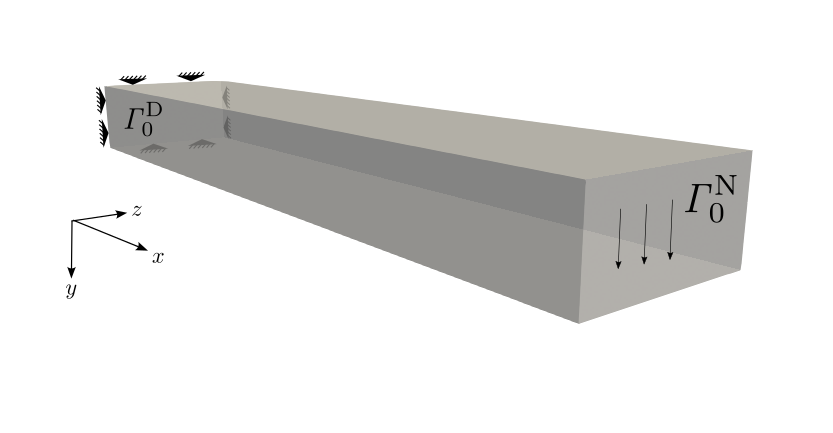
\includegraphics[width=0.7\columnwidth]{fig/cantilever_setup.png}
\caption{Cantilever, problem setup.}
\label{fig_cantilever_setup}
\end{figure}

Study the setup shown in fig. \ref{fig_cantilever_setup} and the comments in the input file \verb"solid_cantilever.py" Run the simulation, either in one of the provided Docker containers or using your own FEniCSx/Ambit installation, using the command

\begin{verbatim}
mpiexec -n 1 python3 solid_cantilever.py
\end{verbatim}

It is fully sufficient to use one core (\verb#mpiexec -n 1#) for the presented setup.

Open the results file \verb"results_solid_cantilever_displacement.xdmf" in Paraview, and visualize the deformation over time.

Figure \ref{fig_cantilever_results} shows the displacement magnitude at the end of the simulation.

\begin{figure}
\centering
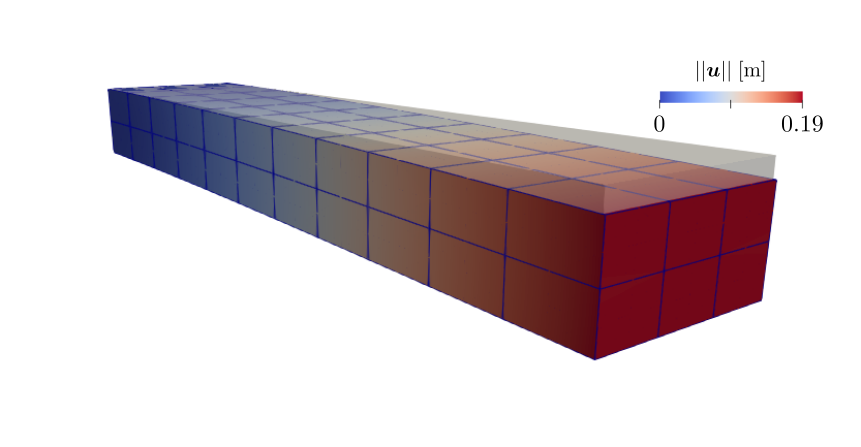
\includegraphics[width=0.7\columnwidth]{fig/cantilever_results}
\caption{Cantilever, tip deformation. Color shows displacement magnitude.}
\label{fig_cantilever_results}
\end{figure}


\subsection{Fluid}\label{subsec_demos_fluid}

- Physics description given in sec. \ref{sec_fluid}

\subsubsection*{2D channel flow}

This example shows how to set up 2D fluid flow in a channel around a rigid obstacle. Incompressible Navier-Stokes flow is solved using Taylor-Hood elements
(9-node biquadratic quadrilaterals for the velocity, 4-node bilinear quadrilaterals for the pressure).

\begin{figure}
\centering
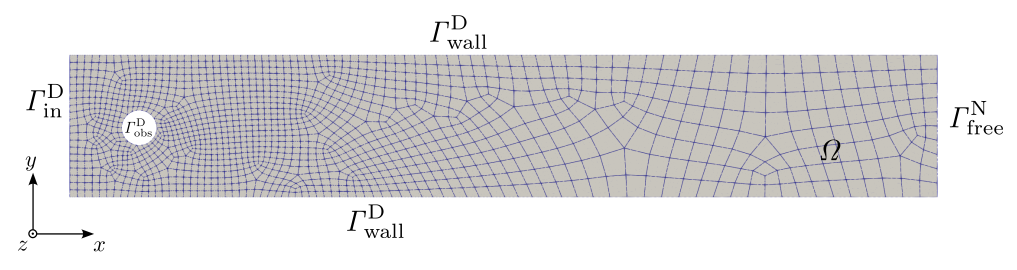
\includegraphics[width=1.0\columnwidth]{fig/channel_setup.png}
\caption{Channel flow, problem setup.}
\label{fig_channel_setup}
\end{figure}

Study the setup and the comments in the input file \verb#fluid_channel.py`#. Run the simulation, either in one of the provided Docker containers or using your own FEniCSx/Ambit installation, using the command

\begin{verbatim}
mpiexec -n 1 python3 fluid_channel.py
\end{verbatim}

It is fully sufficient to use one core (mpiexec -n 1) for the presented setup.

Open the results file \verb"results_fluid_channel_velocity.xdmf" and \\ \verb"results_fluid_channel_pressure.xdmf" in Paraview, and visualize the velocity as well as the pressure over time.

Fig. \ref{fig_channel_results} shows the velocity magnitude (top) as well as the pressure (bottom part) at the end of the simulation.

\begin{figure}[ht]
\centering
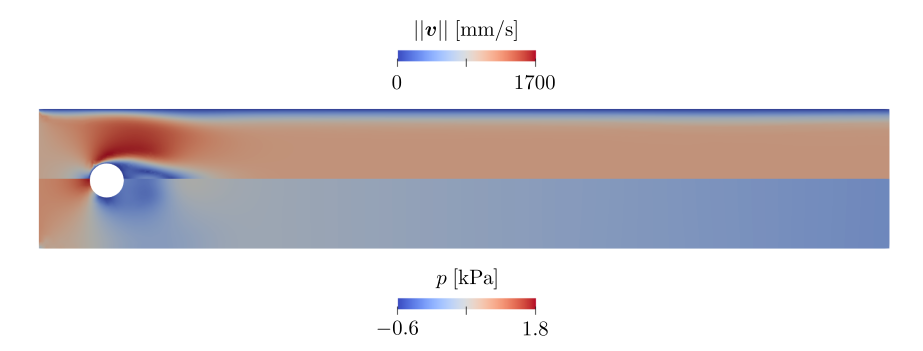
\includegraphics[width=1.0\columnwidth]{fig/channel_results.png}
\caption{Velocity magnitude (top part) and pressure (bottom part) at end of simulation.}
\label{fig_channel_results}
\end{figure}


\subsection{0D flow}\label{subsec_demos_flow0d}

\subsubsection*{Systemic and pulmonary circulation}

This example demonstrates how to simulate a cardiac cycle using a lumped-parameter (0D) model for the heart chambers and the entire circulation. Multiple heart beats are run
until a periodic state criterion is met (which compares variable values at the beginning to those at the end of a cycle, and stops if the relative change is less than
a specified value, here \verb"`eps_periodic'" in the \verb"TIME_PARAMS" dictionary). The problem is set up such that periodicity is reached after 5 heart cycles.

\begin{figure}
\centering
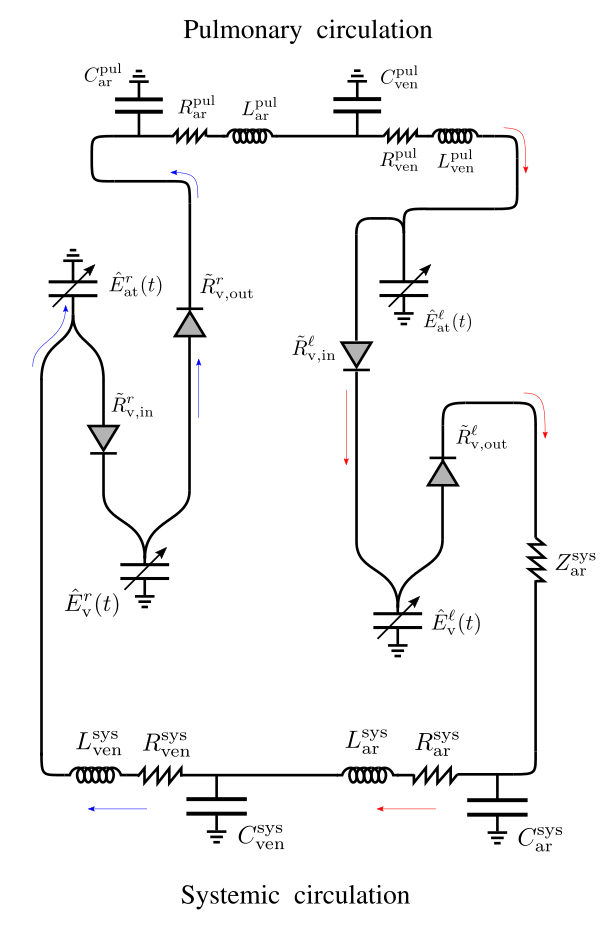
\includegraphics[width=0.5\columnwidth]{fig/syspul_setup.png}
\caption{0D heart, systemic and pulmonary circulation, problem setup.}
\label{fig_syspul_setup}
\end{figure}

Study the setup in fig. \ref{fig_syspul_setup} and the comments in the input file \verb"flow0d_heart_cycle.py". Run the simulation, either in one of the provided Docker containers or using your own FEniCSx/Ambit installation, using the command
\begin{verbatim}
python3 flow0d_heart_cycle.py
\end{verbatim}

For postprocessing of the time courses of pressures, volumes, and fluxes of the 0D model, either use your own tools to plot the text output files (first column is time, second is the respective quantity), or make sure to have Gnuplot (and TeX) installed and navigate to the output folder (\verb"tmp/") in order to execute the script \verb"flow0d_plot.py" (which lies in \verb"ambit/src/ambit_fe/postprocess/"):
\begin{verbatim}
flow0d_plot.py -s flow0d_heart_cycle -n 100
\end{verbatim}
A folder \verb"plot_flow0d_heart_cycle" is created inside \verb"tmp/". Look at the results of pressures ($p$), volumes ($V$), and fluxes ($q$, $Q$) over time.
Subscripts \verb"v", \verb"at", \verb"ar", \verb"ven" refer to `ventricular', `atrial', `arterial', and `venous', respectively. Superscripts \verb"l", \verb"r", \verb"sys", \verb"pul" refer to `left', `right', `systemic', and
`pulmonary', respectively.
Try to understand the time courses of the respective pressures, as well as the plots of ventricular pressure over volume.
Check that the overall system volume is constant and around 4-5 liters.\\

The solution is depicted in fig. \ref{fig_syspul_results}, showing the time course of volumes and pressures of the circulatory system.

\begin{figure}
\centering
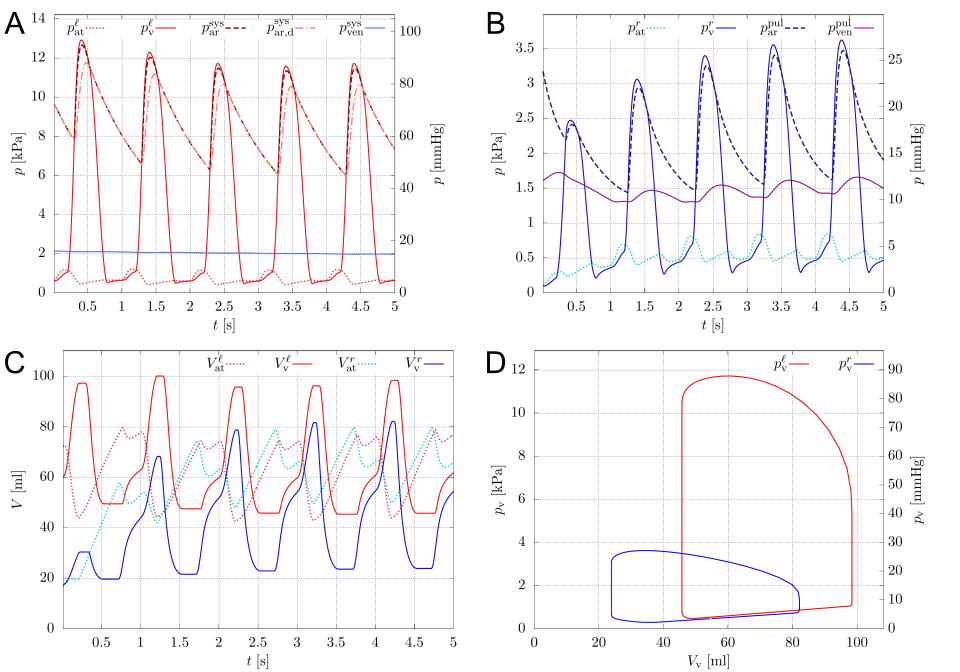
\includegraphics[width=1.0\columnwidth]{fig/syspul_results.png}
\caption{A. Left heart and systemic pressures over time. B. Right heart and pulmonary pressures over time. C. Left and right ventricular and atrial volumes over time. D. Left and right ventricular pressure-volume relationships of periodic (5th) cycle.}
\label{fig_syspul_results}
\end{figure}


\subsection{Solid + 0D flow}\label{subsec_demos:solid_flow0d}

\subsubsection*{3D heart, coupled to systemic and pulmonary circulation}

This example demonstrates how to set up and simulate a two-chamber (left and right ventricular) solid mechanics heart model coupled to a closed-loop
0D circulatory system. A full dynamic heart cycle of duration 1 s is simulated, where the active contraction is modeled by a prescribed active stress approach.
Passive material behavior of the heart muscle is governed by the Holzapfel-Ogden anisotropic strain energy function \cite{holzapfel2009} and a strain rate-dependent viscous model \cite{chapelle2012}.
We start the simulation with "prestressing" using the MULF method \cite{gee2010,schein2021}, which allows to imprint loads without changing the geometry,
where the solid is loaded to the initial left and right ventricular pressures.
Thereafter, we kickstart the dynamic simulation with passive ventricular filling by the systole of the atria (0D chamber models). Ventricular systole
happens in $t \in [0.2 s, 0.53 s]$, hence lasting a third of the whole cycle time. After systole, the heart relaxes and eventually fills to about the same pressure
as it has been initialized to.\\

NOTE: For demonstrative purposes, a fairly coarse finite element discretization is chosen here, which by no means yields a spatially converged solution and which
may be prone to locking phenomena. The user may increse the parameter \verb"`order_disp'" in the \verb"FEM_PARAMS" section from \verb"1" to \verb"2" (and increase \verb"`quad_degree'" to \verb"6") such that quadratic finite element ansatz functions (instead of linear ones) are used. While this will increase accuracy and mitigate locking, computation time will
increase.

\begin{figure}
\centering
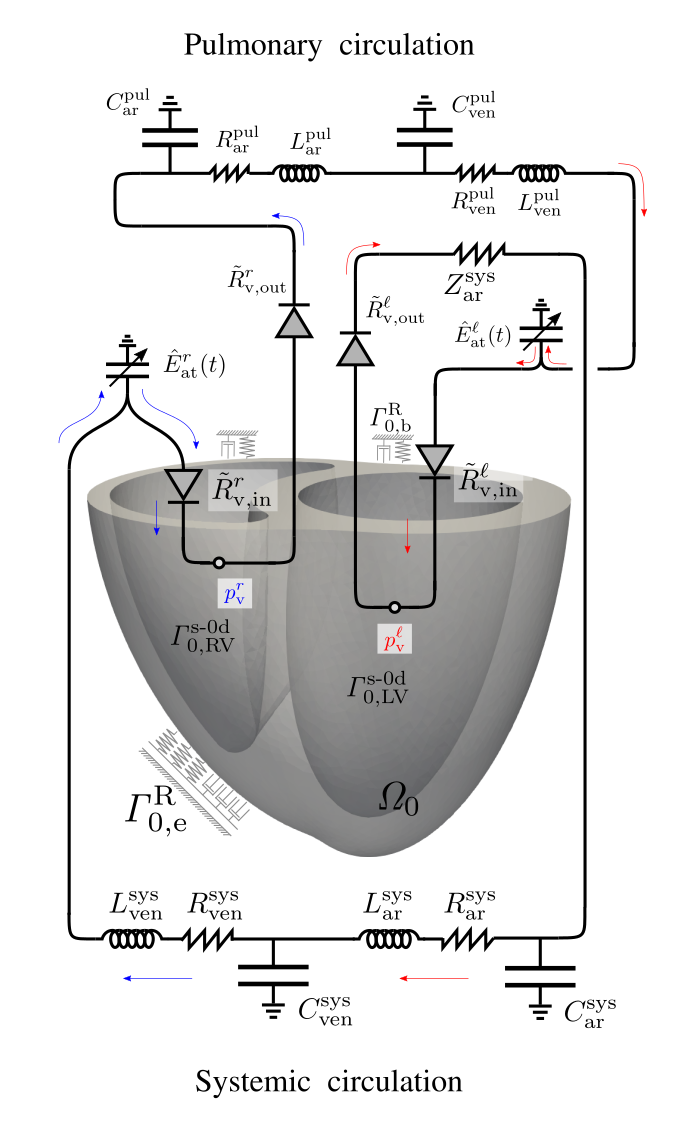
\includegraphics[width=0.6\columnwidth]{fig/heart_syspul_setup.png}
\caption{Generic 3D ventricular heart model coupled to a closed-loop systemic and pulmonary circulation model.}
\label{fig_heart_syspul_setup}
\end{figure}

Study the setup shown in fig. \ref{fig_heart_syspul_setup} and the comments in the input file \verb"solid_flow0d_heart_cycle.py". Run the simulation, either in one of the provided Docker containers or using your own FEniCSx/Ambit installation, using the command
\begin{verbatim}
mpiexec -n 1 python3 solid_flow0d_heart_cycle.py
\end{verbatim}

It is fully sufficient to use one core (\verb"mpiexec -n 1") for the presented setup, while you might want to use more (e.g., \verb"mpiexec -n 4") if you increase \verb"`order_disp'" to \verb"2".

Open the results file \verb"results_solid_flow0d_heart_cycle_displacement.xdmf" in Paraview, and visualize the deformation over the heart cycle.

For postprocessing of the time courses of pressures, volumes, and fluxes of the 0D model, either use your own tools to plot the text output files (first column is time, second is the respective quantity), or make sure to have Gnuplot (and TeX) installed and navigate to the output folder (\verb"tmp/") in order to execute the script \verb"flow0d_plot.py" (which lies in \verb"ambit/src/ambit_fe/postprocess/"):
\begin{verbatim}
flow0d_plot.py -s solid_flow0d_heart_cycle -V0 117e3 93e3 0 0 0
\end{verbatim}

A folder \verb"plot_solid_flow0d_heart_cycle" is created inside \verb"tmp/". Look at the results of pressures ($p$), volumes ($V$), and fluxes ($q$, $Q$) over time.
Subscripts \verb"v", \verb"at", \verb"ar", \verb"ven" refer to `ventricular', `atrial', `arterial', and `venous', respectively. Superscripts \verb"l", \verb"r", \verb"sys", \verb"pul" refer to `left', `right', `systemic', and
`pulmonary', respectively.
Try to understand the time courses of the respective pressures, as well as the plots of ventricular pressure over volume.
Check that the overall system volume is constant and around 4-5 liters.\\

NOTE: This setup computes only one cardiac cycle, which does not yield a periodic state solution (compare e.g. initial and end-cyclic right ventricular pressures and volumes,
which do not coincide). Change the parameter \verb"number_of_cycles" from \verb"1" to \verb"10" and re-run the simulation. The simulation will stop when the cycle error (relative change in 0D variable quantities from beginning to end of a cycle) falls below the value of \verb"`eps_periodic'" (set to $5 \%$). How many cycles are needed to reach periodicity?\\

Figure \ref{fig_heart_syspul_results} shows a high-fidelity solution using a refined mesh and quadratic tetrahedral elements. Compare your solution from the coarser mesh. What is the deviation
in ventricular volume?

\begin{figure}
\centering
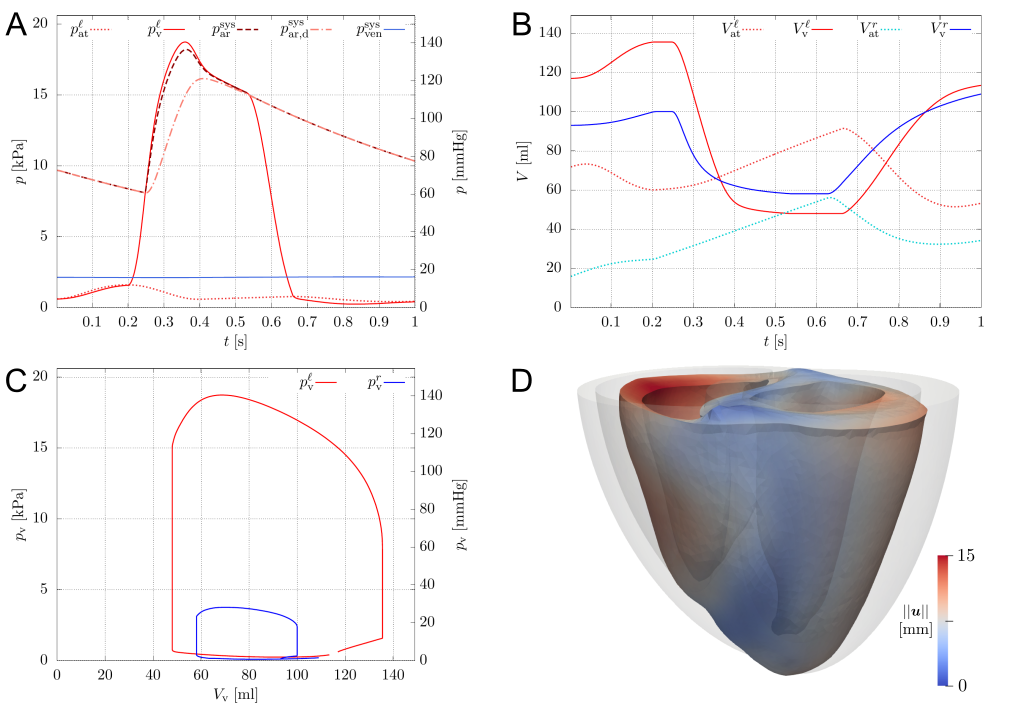
\includegraphics[width=1.0\columnwidth]{fig/heart_syspul_results.png}
\caption{A. Left heart and systemic pressures over time. B. Left and right ventricular and atrial volumes over time. C. Left and right ventricular pressure-volume relationships. D. Snapshot of heart deformation at end-systole, color indicates displacement magnitude.}
\label{fig_heart_syspul_results}
\end{figure}


\subsection{Fluid + 0D flow}\label{subsec_demos:fluid_flow0d}

\subsubsection*{Blocked pipe flow with 0D model bypass}

This example demonstrates how to couple 3D fluid flow to a 0D lumped-parameter model. Incompressible transient Navier-Stokes flow in a pipe with prescibed inflow is solved,
with the special constraint that an internal boundary (all-time closed valve) separates region 1 and region 2 of the pipe. This internal Dirichlet condition can only be achieved
by splitting the pressure space, hence having duplicate pressure nodes at the valve plane. Otherwise, fluid would experience deceleration towards the valve and unphysical acceleration behind it, since the pressure gradient drives fluid flow. To achieve this, the mixed Dolfinx branch instead of the main branch is used. It is installed inside the Ambit devenv Docker
container. In the future, this functionality is expected to be merged into the Dolfinx main branch (at least it was announced...).\\

This example demonstrates how the closed valve can be bypassed by a 0D flow model that links the 3D fluid out-flow of one region to the in-flow of the other region. The 0D model consists of two Windkessel models in series, each having compliance, resistance, and inertance elements.

\begin{figure}
\centering
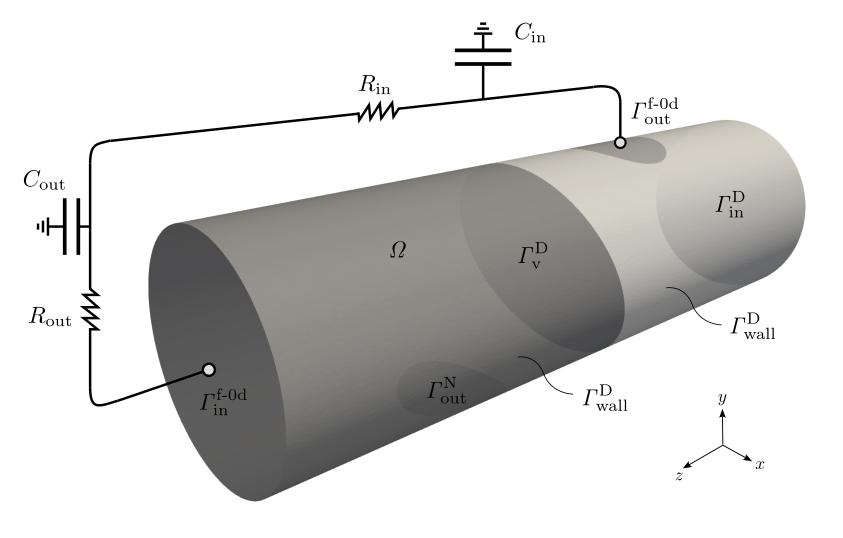
\includegraphics[width=0.8\columnwidth]{fig/pipe_0d_setup.png}
\caption{Blocked pipe with 0D model bypass, simulation setup.}
\label{fig_pipe_0d_setup}
\end{figure}

Study the setup shown in fig. \ref{fig_pipe_0d_setup} and the comments in the input file \verb"fluid_flow0d_pipe.py". Run the simulation, either in one of the provided Docker containers or using your own FEniCSx/Ambit installation, using the command
\begin{verbatim}
mpiexec -n 1 python3 fluid_flow0d_pipe.py
\end{verbatim}
It is fully sufficient to use one core (\verb"mpiexec -n 1") for the presented setup.

Open the results file \verb"results_fluid_flow0d_pipe_velocity.xdmf" in Paraview, and visualize the velocity over time.

Think of which parameter(s) of the 0D model to tweak in order to achieve a) little to no fluid in-flow (into $\mathit{\Gamma}_{\mathrm{in}}^{\mathrm{f\text{-}0d}}$), b) almost the same flow across $\mathit{\Gamma}_{\mathrm{out}}^{\mathrm{f\text{-}0d}}$ and $\mathit{\Gamma}_{\mathrm{in}}^{\mathrm{f\text{-}0d}}$. Think of where the flow is going to in case of a).\\

Figure shows the velocity streamlines and magnitude at the end of the simulation.

\begin{figure}
\centering
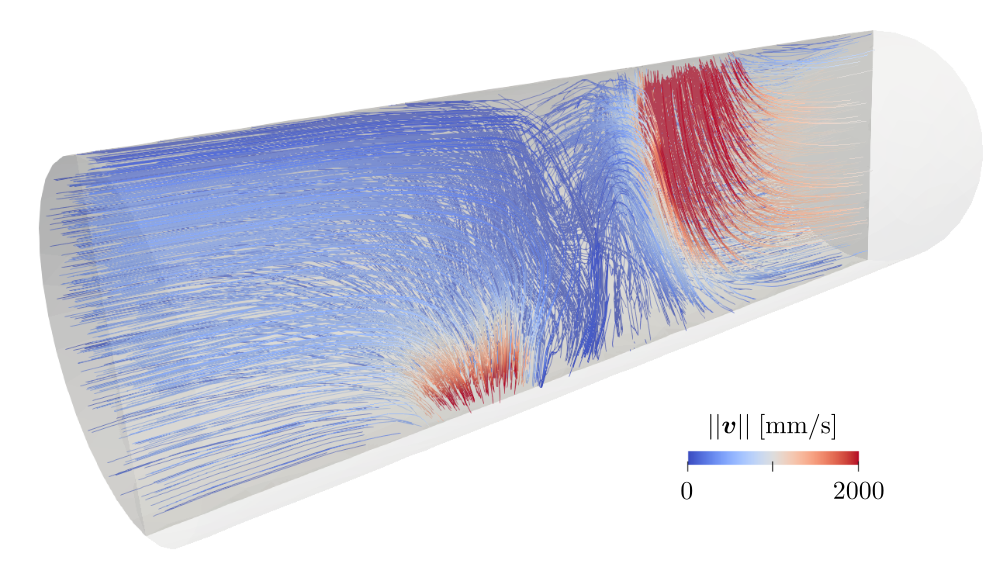
\includegraphics[width=0.7\columnwidth]{fig/pipe_0d_results.png}
\caption{Streamlines of velocity at end of simulation, color indicates velcity magnitude.}
\label{fig_pipe_0d_results}
\end{figure}

\bibliography{ref}

\end{document}
